\documentclass[journal,onecolumn,11pt]{IEEEtran}

\usepackage{iftex}
\ifXeTeX
  \usepackage{fontspec}
  \setmainfont{texgyretermes}[Extension=.otf, UprightFont=*-regular, BoldFont=*-bold, ItalicFont=*-italic, BoldItalicFont=*-bolditalic]
  \setmonofont{texgyrecursor}[Extension=.otf, UprightFont=*-regular, BoldFont=*-bold, ItalicFont=*-italic, BoldItalicFont=*-bolditalic, Scale=0.95]
\else
  \usepackage[utf8]{inputenc}
  \usepackage[T1]{fontenc}
  \usepackage{newtxtext}
\fi
\usepackage{amsmath,amssymb}
\usepackage{graphicx}
\usepackage{booktabs}
\usepackage{tabularx}
\usepackage{multirow}
\usepackage{array}
\usepackage{xcolor}
\usepackage{listings}
\usepackage{algorithm}
\usepackage{algpseudocode}
\usepackage{tikz}
\usetikzlibrary{arrows.meta,positioning,shapes.geometric,fit,calc}
\usepackage[hidelinks]{hyperref}
\usepackage{url}
\usepackage{cite}

\lstset{
  basicstyle=\ttfamily\footnotesize,
  breaklines=true,
  columns=fullflexible,
  frame=single,
  framerule=0.3pt,
  showstringspaces=false,
  captionpos=b
}

\newcommand{\code}[1]{\texttt{#1}}

\begin{document}

\title{TrustTrail: Accountable, Purpose-Bound Attribute Release\\for Privacy-Aware Federated Identity Management}

\author{Vijender~Yadav~(23BCS132),
        Ansh~Hardaha~(23BCS016),
        and~Sourabh~(23BEC055)%
\thanks{The authors are B.Tech.\ students (7th semester) at the Indian Institute of Information Technology Dharwad, Karnataka, India.}}

\markboth{B.Tech.\ Project Report, IIIT Dharwad, 2026}{Yadav \MakeLowercase{\textit{et al.}}: TrustTrail}

\maketitle

\begin{abstract}
In a typical campus single sign-on deployment every service receives the same identifier and a fixed set of personal claims, no release is tied to a stated purpose, and students cannot see who received what. The survey by Werner, Westphall and Westphall shows that accountability and use limitation are among the least covered privacy characteristics in identity management. We present TrustTrail, a disclosure layer beside an unmodified OpenID Connect provider (Keycloak~26). Keycloak caps which of four disclosure profiles a service may obtain and issues per-service pairwise pseudonyms; a custom mapper removes the shared session identifier. TrustTrail is the only source of attribute values. It releases them only under a purpose declaration that the service has signed, which names the attributes, the purpose and a deletion date, and it returns a signed receipt. Releases and refused rule breaks are recorded in a hash-chained ledger whose Merkle roots are anchored in an Ethereum contract, and violations lower the service's tier automatically. On one machine, the layer added a median of 3.2\,ms per login (95\% CI 3.0--3.4\,ms). Conformance tests detected six tamper attacks and 45 scripted violations as designed, with no false positives in 90 honest releases. On the Sepolia test network, anchoring cost 254{,}408 gas per batch whatever its size. TrustTrail provides evidence of what services promised and received. It does not prove deletion, and its protection against the operator covers only history that has already been anchored.
\end{abstract}

\begin{IEEEkeywords}
Federated identity management, privacy, OpenID Connect, pairwise pseudonyms, purpose limitation, accountability, tamper-evident logging, Merkle tree, blockchain anchoring, trust management.
\end{IEEEkeywords}

\section{Introduction}
\label{sec:intro}

\IEEEPARstart{A}{university} runs many online services for its students: a digital library, a learning management system (LMS), an examination portal, and often third-party applications as well. Identity federation and single sign-on (SSO) made this manageable: the student logs in once at an identity provider (IdP), and each service, called a relying party, accepts the IdP's assertion instead of keeping its own password database~\cite{birrell2013federated,ferdous2015dynamic}. Protocols such as SAML~2.0~\cite{saml2core} and OpenID Connect (OIDC)~\cite{oidccore} on top of OAuth~2.0~\cite{rfc6749} are mature, and open-source IdPs such as Keycloak~\cite{keycloakdocs} make SSO cheap to deploy.

SSO solves the login problem. It does little for privacy, and in some ways it makes privacy worse. The project started from a simple question: what does a typical campus SSO configuration actually send to each service? The answer shows three problems.

\emph{Over-release.} The easiest configuration gives every client the same set of claims: name, e-mail address, roll number, department and year. The library needs to know that the borrower is a current student. It does not need the student's name, and it certainly does not need the roll number. Studies of permission systems show that applications routinely ask for more than they need when nothing stops them~\cite{felt2011permissions,chen2014oauth}.

\emph{Linkability.} If the IdP gives every service the same subject identifier, or the same e-mail address, any two services can join their records. Even when identifiers differ, a session identifier shared across clients in one SSO session can link them, as we show in Section~\ref{sec:design}. Unlinkability is one of the three privacy properties that Birrell and Schneider identify for federated identity~\cite{birrell2013federated}, and it is the one that a default deployment gives up first.

\emph{No record and no recourse.} After a release, the student cannot find out which service received which attribute, for what purpose, or until when. If a service later asks for something it never said it needed, nobody notices, and the service keeps the same access as before. Data protection law expects the opposite. The EU General Data Protection Regulation requires that personal data be collected for specified purposes, limited to what is necessary, kept no longer than necessary, and that the controller be able to demonstrate compliance~\cite{gdpr2016}. India's Digital Personal Data Protection Act, 2023 likewise ties processing to a specified purpose and requires erasure once that purpose is no longer served~\cite{dpdp2023}. These are statements about what should happen. A campus IdP gives no evidence of whether it did.

Our starting point was the survey by Werner, Westphall and Westphall, ``Cloud identity management: A survey on privacy strategies''~\cite{werner2017survey}. The survey proposes a taxonomy of nine privacy characteristics for identity management (transparency, controllability, minimization, accountability, data quality, use limitation, user-friendliness, trust and obfuscation), maps 23 published proposals and six European research projects against it, and lists open challenges. Reading its tables closely, we found that the two characteristics that matter most for the third problem are also the least covered. Only 2 of the 23 proposals address accountability and only 5 address use limitation; the four works the authors themselves present as solutions in progress address neither~\cite[Tables~2--3]{werner2017survey}. The survey also names ``ensure the implementation of policies'' as an open challenge and observes that several surveyed proposals were never implemented or validated. Section~\ref{sec:basepaper} analyses the survey in detail.

This paper presents \emph{TrustTrail}, a system that addresses these gaps for an OIDC federation and that we built and evaluated end to end. TrustTrail keeps the IdP unmodified in its protocol behaviour and adds a disclosure layer beside it. Its design follows one loop:
\begin{center}
\emph{signed promise $\rightarrow$ ledger record $\rightarrow$ violation detected $\rightarrow$ trust lowered $\rightarrow$ less data released.}
\end{center}
A service first signs a purpose declaration that names the attributes it wants, why it wants them and when it will delete them. TrustTrail releases attribute values only under such a declaration and only up to the disclosure profile that the service's current trust tier allows. Every release, and every refused request that breaks a rule, becomes an entry in a hash-chained ledger. Batches of ledger entries are summarised as Merkle roots and anchored in an Ethereum smart contract, so the history cannot be quietly rewritten even by the operator. A service that breaks a rule loses trust, and the IdP stops granting it the more revealing profiles.

\begin{figure}[t]
\centering
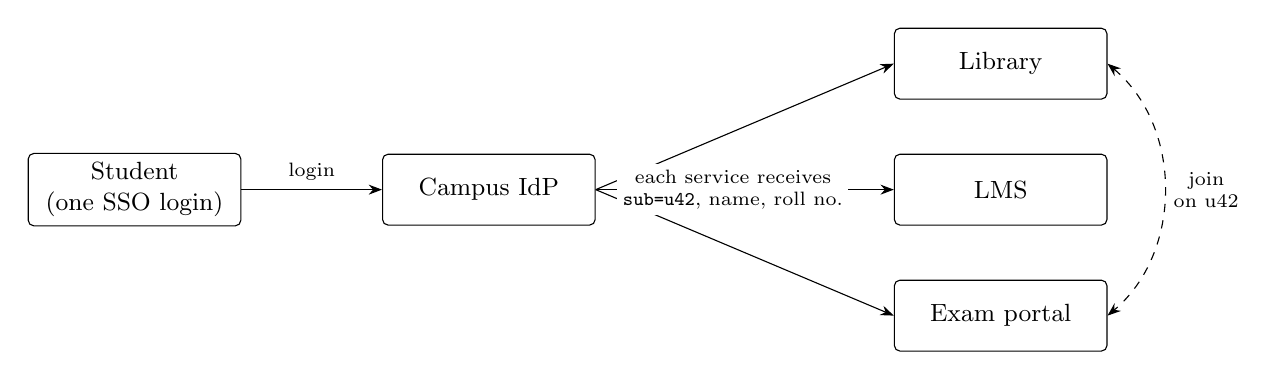
\begin{tikzpicture}[
  box/.style={draw, rounded corners=2pt, align=center, minimum width=27mm, minimum height=9mm, font=\small},
  lab/.style={font=\scriptsize, align=center}]
\node[box] (st) at (0,0) {Student\\(one SSO login)};
\node[box] (idp) at (4.5,0) {Campus IdP};
\node[box] (lib) at (11,1.6) {Library};
\node[box] (lms) at (11,0) {LMS};
\node[box] (exam) at (11,-1.6) {Exam portal};
\draw[-{Stealth}] (st) -- node[lab, above] {login} (idp);
\draw[-{Stealth}] (idp.east) -- (lib.west);
\draw[-{Stealth}] (idp.east) -- (lms.west);
\draw[-{Stealth}] (idp.east) -- (exam.west);
\node[lab, fill=white, inner sep=2pt] at (7.6,0) {each service receives\\\code{sub=u42}, name, roll no.};
\draw[dashed, {Stealth}-{Stealth}] (lib.east) to[bend left=50] node[lab, right] {join\\on u42} (exam.east);
\end{tikzpicture}
\caption{The problem in a default SSO deployment. Every service receives the same identifier and the same personal claims, whatever it needs, so services can join their records; the student has no record of the releases.}
\label{fig:problem}
\end{figure}

\subsection{Research questions}
We framed the work around five questions.
\begin{enumerate}
\item[\textbf{RQ1}] Can a federation give each service only the attributes of an agreed disclosure profile, and stop services from linking a student across services, while the IdP keeps speaking standard OIDC?
\item[\textbf{RQ2}] Can every release be bound to a purpose and a deletion date that the service has signed, so that a service cannot later deny what it promised?
\item[\textbf{RQ3}] Can the record of releases be made tamper-evident against an insider who controls the database, including the operator, without putting personal data on a public ledger?
\item[\textbf{RQ4}] Can rule-breaking that the disclosure layer can observe automatically reduce what the offending service receives in future?
\item[\textbf{RQ5}] What do these mechanisms cost in login latency and in blockchain fees?
\end{enumerate}

\subsection{Contributions}
\begin{enumerate}
\item A gap analysis of Werner et al.~\cite{werner2017survey} that uses the survey's own tables to show where its taxonomy is least covered, and that maps each of its five open challenges to a concrete design requirement (Section~\ref{sec:basepaper}).
\item A design that splits disclosure between the IdP and a separate release service: Keycloak decides \emph{which} profile a service may obtain, using per-service scope assignment as a tier cap, pairwise subject identifiers and a custom protocol mapper that removes the shared session identifier; TrustTrail decides \emph{what} the profile contains and is the only path for attribute values (Sections~\ref{sec:architecture} and~\ref{sec:design}).
\item Signed purpose declarations and release receipts based on JSON Web Signatures~\cite{rfc7515}, which bind every release to the attributes, purpose and deletion date that the service promised, and give the student portable, verifiable evidence of each release.
\item An accountability chain made of a hash-chained ledger, per-release receipts and Merkle-root anchoring in an Ethereum contract that only accepts contiguous batches, with a verification procedure that a student can run using only a downloaded receipt and the chain.
\item A dynamic trust model in which three observable violation rules lower a service's score and its tier, and the tier is enforced both at the IdP (login is refused) and at the release service (already issued tokens get the lower cap).
\item An open implementation (Keycloak~26.8.1, Python~3.12/FastAPI, Solidity~0.8.28, Hardhat~3) with 149 Python tests and 6 contract tests, and an evaluation of latency, tamper detection, violation detection and anchoring cost (Sections~\ref{sec:implementation} and~\ref{sec:evaluation}).
\end{enumerate}

We are careful about what TrustTrail does not do. It records what a service promised and what it received, and it refuses releases that break the promise. It cannot see what a service does with data afterwards, so it cannot prove deletion. The IdP still sees every login. Section~\ref{sec:discussion} discusses these and other limits.

\subsection{Organisation}
Section~\ref{sec:background} introduces the protocols and primitives that TrustTrail builds on. Section~\ref{sec:basepaper} analyses the base survey and derives the gaps we address, and Section~\ref{sec:related} reviews related work. Section~\ref{sec:threat} states the threat model and design goals. Sections~\ref{sec:architecture} and~\ref{sec:design} present the architecture and the detailed design, and Section~\ref{sec:implementation} the implementation. Section~\ref{sec:evaluation} reports the evaluation. Sections~\ref{sec:discussion}, \ref{sec:future} and~\ref{sec:conclusion} discuss limitations, future work and conclusions.

\section{Background}
\label{sec:background}

This section introduces the protocols, cryptographic building blocks and privacy principles that the rest of the paper relies on. Readers familiar with OIDC and Merkle trees can skip to Section~\ref{sec:basepaper}.

\subsection{Identity management, federation and single sign-on}
Identity management (IdM) covers how identities are created, authenticated, described by attributes and eventually removed. In a federation, several organisations agree to trust each other's identity assertions. One party, the identity provider (IdP), authenticates the user and issues an assertion; the service provider (SP), or relying party (RP) in OIDC terms, accepts the assertion and makes its own authorisation decision~\cite{werner2017survey,birrell2013federated}. Single sign-on (SSO) follows: once the user has a session at the IdP, further services can be reached without logging in again.

Federations differ in how much the members trust each other. Ferdous and Poet distinguish \emph{fully trusted}, \emph{semi-trusted} and \emph{untrusted} entities in dynamic SAML federations, depending on whether a legal agreement backs the relationship~\cite{ferdous2015dynamic}. TrustTrail reuses these three names for its service tiers and adds a fourth, \emph{blocked}, for services that have lost trust through violations.

From a privacy point of view, the IdP is in a powerful position. It knows every user's attributes and sees every login to every service. Birrell and Schneider characterise federated IdM systems by three properties that users may want~\cite{birrell2013federated}: \emph{undetectability} (others cannot tell that a transaction happened), \emph{unlinkability} (transactions cannot be connected to each other or to the user) and \emph{confidentiality} (the user controls who learns their attributes). Pfitzmann and Hansen give the standard terminology for anonymity, unlinkability and pseudonymity~\cite{pfitzmann2010terminology}. A \emph{pseudonym} is an identifier other than the user's real name; it is \emph{relationship-specific} when the user has a different pseudonym for each communication partner, which prevents partners from linking the user by identifier.

\subsection{OAuth 2.0 and OpenID Connect}
OAuth~2.0~\cite{rfc6749} lets a client obtain an \emph{access token} from an authorisation server in order to call a protected API. The client asks for \emph{scopes}, which name the permissions it wants, and the server decides which scopes to grant. Two OAuth flows matter here. In the \emph{authorization code} flow, the user's browser is redirected to the server, the user authenticates, and the client exchanges a one-time code for tokens over a back channel. In the \emph{client credentials} flow, a client authenticates as itself, with no user involved; TrustTrail uses it to authenticate services that register their keys.

OpenID Connect~\cite{oidccore} adds authentication on top of OAuth. The server, now an OpenID Provider, issues an \emph{ID token}: a signed JSON Web Token (JWT)~\cite{rfc7519} whose claims state who the user is (\code{sub}), who issued the token (\code{iss}), for which client it is meant (\code{aud}) and when it was issued and expires. Additional user attributes, such as name or e-mail address, can be placed in the ID token, the access token, or returned from a userinfo endpoint, depending on the requested scopes and the provider's configuration. Keycloak~\cite{keycloakdocs} controls this per client through \emph{client scopes} and \emph{protocol mappers}. A client scope bundles claims; it can be assigned to a client as a \emph{default} scope (always granted) or an \emph{optional} scope (granted only when requested). A protocol mapper is a plug-in that adds, changes or removes claims in the tokens that a client receives.

\subsubsection{Pairwise subject identifiers}
OIDC defines two subject identifier types~\cite[Sec.~8]{oidccore}. With the \emph{public} type, every client receives the same \code{sub} for a user. With the \emph{pairwise} type, each client, or more exactly each \emph{sector} of clients, receives a different \code{sub}, so clients cannot correlate the user by identifier. The specification suggests computing the pairwise value as a hash of the sector identifier, the local account identifier and a secret salt. Keycloak's SHA-256 pairwise mapper does this and then formats the 32-byte digest as a name-based (version~3) UUID; the sector is the host name of the client's redirect URIs unless a sector identifier URI is configured. Pairwise identifiers are also recommended by NIST's federation guidelines~\cite{nist80063c}.

\subsubsection{Session identifiers}
Keycloak adds a session identifier claim, \code{sid}, to the tokens it issues. All clients that a user reaches within one SSO session receive the same \code{sid} value. The authorisation response can also carry a \code{session\_state} parameter derived from the session. As Section~\ref{sec:design} shows, these values defeat pairwise identifiers: two services that compare \code{sid} values can link the two pseudonyms of the same student.

\subsection{JSON Web Signatures and keys}
A JSON Web Signature (JWS)~\cite{rfc7515} protects a payload with a digital signature or MAC. Its \emph{compact serialisation} is three base64url strings separated by dots: a protected header, the payload and the signature. The header names the algorithm (\code{alg}), may name the signing key (\code{kid}) and may state a media type (\code{typ}) so that a JWS meant for one purpose is not accepted for another. TrustTrail uses two algorithms from the JSON Web Algorithms specification~\cite{rfc7518}: ES256 (ECDSA on curve P-256 with SHA-256) and RS256 (RSASSA-PKCS1-v1\_5 with SHA-256). Public keys are exchanged as JSON Web Keys (JWK)~\cite{rfc7517}. The JWK thumbprint~\cite{rfc7638} is the SHA-256 hash of a canonical JSON object made of the key's required members in lexicographic order; it gives a key a stable identifier that is derived from the key itself, which TrustTrail uses as the \code{kid}.

A signed JWS gives \emph{non-repudiation} in a practical sense: if the verifier keeps the JWS, it can later show a third party that the holder of the private key signed exactly this payload. TrustTrail relies on this property for purpose declarations, which services sign, and for release receipts, which TrustTrail signs.

\subsection{Hash chains and tamper-evident logs}
A cryptographic hash function such as SHA-256 maps any input to a fixed-size digest; it is infeasible to find two inputs with the same digest or to change an input without changing its digest. A \emph{hash chain} links records by including the digest of the previous record in each new record. Haber and Stornetta used this idea to timestamp digital documents~\cite{haber1991timestamp}, and Schneier and Kelsey applied it to audit logs, so that an attacker who takes over a logging machine cannot undetectably change entries written before the takeover~\cite{schneier1999secure}. A chain alone has a known weakness: whoever controls the whole log can rewrite an entry and recompute every later hash, or cut off the newest entries. Detecting that requires some value that the attacker cannot change, such as a hash that has been published elsewhere or handed to a third party~\cite{crosby2009efficient,ma2007forward}.

\subsection{Merkle trees}
A Merkle tree~\cite{merkle1987signature} hashes a list of items in pairs, then hashes the results in pairs, until one \emph{root} hash remains. The root commits to every item and its position. To prove that an item is in the tree, it is enough to give the hashes of its siblings on the path to the root, which takes $\lceil \log_2 n \rceil$ hashes for $n$ items; the verifier recomputes the root and compares. Certificate Transparency (CT) uses Merkle trees for public, append-only logs of TLS certificates~\cite{laurie2014certificate}. Its specification, RFC~6962~\cite{rfc6962} (updated by RFC~9162~\cite{rfc9162}), prefixes leaf inputs with the byte \code{0x00} and interior-node inputs with \code{0x01}. This domain separation stops an attacker from presenting an interior node as a leaf. TrustTrail follows these conventions.

\subsection{Blockchains, smart contracts and anchoring}
A blockchain is a replicated ledger in which blocks of transactions are linked by hashes and agreed on by many independent nodes, so that a confirmed transaction is very hard to remove or change~\cite{nakamoto2008bitcoin}. Ethereum~\cite{wood2014ethereum} adds \emph{smart contracts}: programs stored on the chain whose functions are called by transactions. A contract can keep state, emit \emph{events} that clients can search, and reject calls that break its rules. Every operation costs \emph{gas}, paid for in the chain's currency; writing to contract storage is among the most expensive operations. Contracts are usually written in Solidity~\cite{soliditydocs} and tested on a local development chain such as Hardhat~\cite{hardhatdocs} before deployment to a public test network such as Sepolia or to the main network.

\emph{Anchoring} uses a blockchain as the external, hard-to-change place where a log's hash is published. Instead of writing each record, a system periodically writes one Merkle root that covers many records. OpenTimestamps~\cite{todd2016opentimestamps} and Chainpoint~\cite{chainpoint} anchor document hashes this way. Anchoring keeps the data off chain, which matters for personal data that must not become public and permanent, and keeps the cost per record low.

\subsection{Privacy principles in law and design}
The GDPR~\cite{gdpr2016} lists principles for processing personal data in Article~5. Four of them shape TrustTrail's goals: \emph{purpose limitation} (data is collected for specified, explicit purposes), \emph{data minimisation} (adequate, relevant and limited to what is necessary), \emph{storage limitation} (kept no longer than necessary) and \emph{accountability} (the controller is responsible for, and able to demonstrate, compliance). India's Digital Personal Data Protection Act, 2023~\cite{dpdp2023} applies to student data held by Indian institutes; it likewise links processing to a specified purpose and requires erasure when the purpose is no longer served. Cavoukian's \emph{Privacy by Design} principles~\cite{cavoukian2011pbd} ask that privacy be the default setting, embedded into the design, and visible and transparent to the user. The Kantara Initiative's Consent Receipt specification~\cite{kantarareceipt} proposes giving users a record of each consent they grant, an idea close to TrustTrail's release receipts.

Table~\ref{tab:terms} summarises the terms used in the rest of the paper.

\begin{table}[t]
\centering
\caption{Terms used in this paper}
\label{tab:terms}
\small
\begin{tabularx}{\linewidth}{@{}l X@{}}
\toprule
Term & Meaning in TrustTrail \\
\midrule
IdP & Keycloak, the campus OpenID Provider. Authenticates students and issues tokens. \\
Service & A relying party, such as the library, the LMS or the exam portal. \\
Profile & One of four disclosure levels: \emph{anonymous}, \emph{pseudonym}, \emph{partial}, \emph{total}. Each maps to a fixed attribute set. \\
Tier & A service's trust level: \emph{fully\_trusted}, \emph{semi\_trusted}, \emph{untrusted} or \emph{blocked}. Each tier has a profile cap. \\
Base tier & The tier in the service's agreement with the institute; its cap is the most the service may ever ask for. \\
Pairwise \code{sub} & The per-service pseudonym of a student. \\
Purpose declaration & A JWS signed by a service: attributes, purpose, deletion date (\code{retention\_until}). \\
Release & One delivery of attribute values from TrustTrail to a service. \\
Receipt & A JWS signed by TrustTrail that describes one release. \\
Ledger & The append-only, hash-chained table of releases, violations and trust resets. \\
Violation & A refused request that breaks one of three rules; recorded in the ledger and counted against trust. \\
Anchor & A Merkle root of a contiguous batch of ledger entries, stored in the \code{TrustTrailAnchor} contract. \\
\bottomrule
\end{tabularx}
\end{table}

\section{The Base Paper and Its Gaps}
\label{sec:basepaper}

TrustTrail is a follow-up to the survey by Werner, Westphall and Westphall~\cite{werner2017survey}, published in \emph{Computer Networks} in 2017. This section summarises what the survey contributes, reads its tables quantitatively, and derives the gaps that TrustTrail addresses. All counts below come from the survey's own tables; we did not re-score the surveyed works.

\subsection{What the survey does}
The survey starts from the observation that, even with IdM systems, ``leakage of user data, the distribution of unnecessary attributes, and a lack of control on the dissemination of personal data are recurrent in cloud environments''~\cite{werner2017survey}. It asks three research questions: which IdM model is needed to ensure privacy in cloud computing, which techniques best address the lack of privacy control in interactions, and how federation partners should agree on privacy for authentication and authorisation. To answer them, the authors ran a systematic mapping. A keyword search found 198 papers, which were filtered by title and abstract and then by content.

The central contribution is a taxonomy of privacy characteristics for IdM in the cloud, shown as a mind map in the survey's Fig.~3. It has nine characteristics, each refined into two mechanisms:
\begin{itemize}
\item \emph{Transparency} (advertence, consciousness): the user is told how attributes are collected, used and disclosed.
\item \emph{Controllability} (selection, consent): the user chooses what is released and agrees to it.
\item \emph{Minimization} (control, participation): only the information needed to access a resource is released.
\item \emph{Accountability} (traceability, policies): auditing and tracking actions, ``in accordance with legal requirements'', so that misuse and privacy breaches can be identified and audited.
\item \emph{Data quality} (validation, confidence): attributes are correct and validated.
\item \emph{Use limitation} (obligations, policies): only authorised entities use the data, for the stated reason; a policy can state ``the reason or intention for using the data'' and an obligation is a directive to be carried out before or after access.
\item \emph{User-friendliness} (with or without add-ons): an interface lets users ``check what data was released under what conditions, and to whom''.
\item \emph{Trust} (reputation, risk): confidence in providers is assessed with metrics.
\item \emph{Obfuscation} (anonymity, pseudonym): users are not identified, or are identified only by pseudonyms.
\end{itemize}
The survey relates these characteristics to the three properties of Birrell and Schneider (confidentiality, undetectability, unlinkability) in a Venn diagram (its Fig.~4).

The survey then classifies six European research projects (PRIME, PrimeLife, ABC4Trust, GÉANT, PRISMACLOUD and CREDENTIAL; its Table~1) and 23 published proposals from 2009 to 2016 (its Table~2) by the characteristics they address. It describes five challenges for future research (its Section~4) and four works in progress by the authors' group (its Section~5 and Table~3). One of these works defines four standard \emph{interaction profiles}, anonymous, pseudonym, partial attributes and total attributes, as OIDC scopes~\cite{werner2015approach}; another adds a dissemination screen that warns the user about the provider's reputation~\cite{werner2016model}.

\subsection{Reading the tables}
Table~\ref{tab:coverage} counts how many of the surveyed proposals and projects address each characteristic. Two characteristics stand out. Accountability is marked for only 2 of the 23 proposals (Suriadi et al.~\cite{suriadi2009usercentric} and Sánchez et al.~\cite{sanchez2012enhancing}) and for 3 of the 6 projects. Use limitation is marked for 5 proposals and 2 projects. Data quality and user-friendliness are also rare, but they are less central to the problems described in Section~\ref{sec:intro}. In the authors' own works in progress, accountability and use limitation are not marked for any of the four.

\begin{table}[t]
\centering
\caption{Coverage of the nine privacy characteristics in the survey by Werner et al.~\cite{werner2017survey}, counted from its Tables~1--3}
\label{tab:coverage}
\small
\begin{tabular}{@{}lccc@{}}
\toprule
Characteristic & Proposals (of 23, Table 2) & EU projects (of 6, Table 1) & Authors' works (of 4, Table 3) \\
\midrule
Transparency     & 14 & 6 & 4 \\
Controllability  & 17 & 6 & 3 \\
Minimization     &  8 & 3 & 1 \\
Accountability   & \textbf{2} & 3 & \textbf{0} \\
Data quality     &  2 & 6 & 1 \\
Use limitation   & \textbf{5} & 2 & \textbf{0} \\
User-friendly    &  2 & 3 & 3 (all ``partial'') \\
Trust            &  5 & 2 & 2 \\
Obfuscation      &  6 & 3 & 1 \\
\bottomrule
\end{tabular}
\end{table}

The numbers suggest a pattern. Most work concentrates on the moment of disclosure: telling the user what will be released (transparency), letting the user choose (controllability) and releasing less (minimization). Far less work addresses what happens around and after the disclosure: whether the release can be traced and audited later (accountability), and whether the service's use is bound to a stated reason and time (use limitation). For students, these are exactly the missing pieces. A student who never sees a record of releases cannot exercise any control after the fact, and a promise of deletion that nobody records cannot be checked.

\subsection{The survey's open challenges}
The survey's Section~4 lists five challenges and directions for privacy-based IdM in the cloud. We summarise each and note what is still open.

\emph{Reliability assessment} (Section~4.1 of the survey). Federation partners need a way to evaluate trust in each other, for example through provider reputation or risk metrics. The surveyed works that address trust mostly use reputation values or static trust levels, such as the fully trusted, semi-trusted and untrusted classes of Ferdous and Poet~\cite{ferdous2015dynamic}. What is missing is a link from observed behaviour to the trust level: a provider that misbehaves keeps its level until someone changes it.

\emph{Agreement of privacy options} (Section~4.2). The IdP and the service should agree in advance on the privacy features of their interaction, and the agreement should not be static. In the surveyed works, such agreements are policies or contracts outside the protocol. They are not bound to individual releases, and the service does not sign anything that could later be held against it.

\emph{Definition of interaction profiles} (Section~4.3). Predefined profiles help users and services disclose the least information needed. The authors' own work defines the four profiles as OIDC scopes~\cite{werner2015approach}. A profile scope says what the service \emph{asks} for. On its own it does not stop a service from asking for a more revealing profile, and it does nothing about linkage across services through identifiers or session values.

\emph{Granular control over the dissemination of data} (Section~4.4). Releasing individual attributes, not whole profiles, should be possible depending on context. This is largely solved by attribute filtering and consent screens in existing systems such as the Shibboleth extension of Orawiwattanakul et al.~\cite{orawiwattanakul2010user}.

\emph{Ensuring the implementation of policies} (Section~4.5). The survey states that ``it is essential that the application of different privacy policies be guaranteed in an automated way'' and calls compliance assessment ``a key challenge''~\cite{werner2017survey}. Sticky policies~\cite{pearson2011sticky,chadwick2012privacy} attach usage conditions to data, but the survey notes about one sticky-policy approach that it ``does not make clear the means to ensure the effective implementation of sticky policies after receiving data''.

\subsection{Weaknesses of the surveyed approaches}
Taken together with the coverage counts, the survey's own remarks point to four weaknesses in the state of the art it describes.

\begin{enumerate}
\item \emph{No evidence trail.} Accountability is the least covered characteristic. Even where it is marked, the works audit the system or trace data inside a trusted environment; none gives the user, or an outside auditor, evidence of releases that the operator cannot later alter.
\item \emph{Purposes without enforcement.} Use limitation appears as policies and obligations, but not as a promise that is checked on every release. A service's purpose and retention period are not recorded with the data that was released under them.
\item \emph{Static trust.} Trust levels and reputation scores are inputs set by administrators or by user feedback; a provider that breaks its promises does not automatically get less data.
\item \emph{Proposals without implementations.} The survey itself observes of several works that they do ``not provide details and [do] not validate the proposal'', offer ``mathematical and logical evidences, without a practical implementation'', or do ``not make clear how to implement'' a component~\cite{werner2017survey}. Several of the works are also built on SAML federations, whereas current campus deployments increasingly use OIDC.
\end{enumerate}

\subsection{From gaps to requirements}
Table~\ref{tab:gaps} maps each challenge and weakness to a requirement for TrustTrail and to the mechanism that meets it. The mechanisms are described in Sections~\ref{sec:architecture} and~\ref{sec:design}, and Section~\ref{sec:eval-taxonomy} compares TrustTrail with the authors' works on the same nine characteristics.

\begin{table}[t]
\centering
\caption{From the survey's challenges to TrustTrail's requirements and mechanisms}
\label{tab:gaps}
\small
\begin{tabularx}{\linewidth}{@{}>{\raggedright\arraybackslash}p{3.2cm} >{\raggedright\arraybackslash}X >{\raggedright\arraybackslash}X@{}}
\toprule
Challenge or weakness & Requirement for TrustTrail & Mechanism \\
\midrule
Reliability assessment (4.1); static trust & Trust must follow observed behaviour and change what a service receives. & Trust score lowered by violations; tier cap enforced at Keycloak and at release (Sec.~\ref{sec:design-trust}). \\
Agreement of privacy options (4.2); purposes without enforcement & The service must commit to attributes, purpose and deletion date before any release, in a form it cannot later deny. & Signed purpose declarations; releases refused outside them; signed receipts (Sec.~\ref{sec:design-declarations}). \\
Interaction profiles (4.3) & The IdP and the release service must both enforce the profile, and services must not be able to link students. & Keycloak scope assignment as tier cap; pairwise \code{sub}; \code{sid} removed by a custom mapper (Sec.~\ref{sec:design-profiles}). \\
Granular control (4.4) & A service may ask for a subset of its profile. & Per-request attribute list checked against declaration and profile (Sec.~\ref{sec:design-declarations}). \\
Ensuring policy implementation (4.5); no evidence trail & Every release and every rule break must be recorded so that later changes are detectable, even by the operator. & Hash-chained ledger, receipts, Merkle anchoring on Ethereum (Secs.~\ref{sec:design-ledger}, \ref{sec:design-anchoring}). \\
Proposals without implementations & The design must run on a current IdP and be measured. & Keycloak 26 implementation, 155 tests, evaluation (Secs.~\ref{sec:implementation}, \ref{sec:evaluation}). \\
\bottomrule
\end{tabularx}
\end{table}

One requirement from the survey we deliberately do not take on. The survey lists data quality, the validation of attribute values, as a characteristic. In a campus federation the IdP is the institute's own system of record, so we treat its attribute values as correct and do not add validation.

\section{Related Work}
\label{sec:related}

Section~\ref{sec:basepaper} covered the works classified in the base survey. This section looks at work beyond the survey, grouped by the problem each line of work solves, and positions TrustTrail against it. Table~\ref{tab:related} summarises the comparison.

\subsection{Privacy-preserving single sign-on}
A standard OIDC provider learns every service that a user logs in to, which lets the IdP build a profile of the user's activity. Several designs remove this. SPRESSO by Fett, Küsters and Schmitz is a web SSO system in which the IdP does not learn which relying party the user logs in to~\cite{fett2015spresso}. Hammann, Sasse and Basin propose a privacy-preserving extension of OIDC with the same aim~\cite{hammann2020privacy}, and Kroschewski and Lehmann address how a relying party can be authenticated in OIDC without revealing it to the IdP~\cite{kroschewski2023implicit}. UPPRESSO, so far available as a preprint, aims at SSO that is both untraceable by the IdP and unlinkable across relying parties~\cite{guo2021uppresso}. On the security side, Fett et al.\ gave a formal analysis of OAuth~2.0~\cite{fett2016oauth}, Mainka et al.\ systematised attacks on OIDC~\cite{mainka2017sok}, and Wang, Chen and Wang showed through traffic analysis that deployed SSO systems had serious logic flaws~\cite{wang2012signing}.

These works protect the user from the IdP, or protect the protocol from attackers. TrustTrail addresses a different question: what the relying parties receive, under which promise, and whether that can be checked later. The two concerns are complementary. In a campus federation the IdP is the institute itself and already holds the student's records, so IdP tracking is less of a concern than over-release to the many services around it. We list IdP tracking as a non-goal in Section~\ref{sec:threat}; a deployment that needs both could combine TrustTrail with one of these protocols.

\subsection{Anonymous credentials and self-sovereign identity}
Chaum proposed in 1985 that individuals use a different pseudonym with each organisation and prove facts about themselves with credentials that cannot be linked across organisations~\cite{chaum1985security}. Camenisch and Lysyanskaya gave an efficient anonymous credential system~\cite{camenisch2001efficient}, which IBM implemented as Idemix~\cite{camenisch2002idemix}; Microsoft's U-Prove offers similar selective disclosure~\cite{paquin2013uprove}. The PRIME, PrimeLife and ABC4Trust projects in the base survey built on these systems. More recently, self-sovereign identity places credentials in a wallet controlled by the user~\cite{allen2016path,muhle2018survey}, and the W3C Verifiable Credentials data model standardises their format~\cite{w3cvc2}.

Credential systems give strong unlinkability and fine-grained disclosure, often stronger than pairwise identifiers, because even the issuer cannot link presentations. They also move work to the user: the student needs a wallet, and every service needs a verifier. More importantly for our goals, a credential presentation leaves no record that the user can later show to a third party, and nothing ties the verifier's use of the data to a declared purpose. TrustTrail takes the opposite trade-off. It keeps standard OIDC on the service side and gives up some unlinkability (the institute's IdP and TrustTrail know the mapping between pseudonyms), in exchange for a central point where purpose, retention and the release record can be enforced and kept.

\subsection{Policy-based control of disclosure}
A large part of the base survey concerns policies that state how released data may be used. Sticky policies attach machine-readable usage conditions to data so that the conditions travel with it~\cite{pearson2011sticky}. Chadwick and Fatema built a privacy-preserving authorisation system in which users' policies are stuck to their data and enforced by the cloud provider's policy decision points~\cite{chadwick2012privacy}. Orawiwattanakul et al.\ let users filter which attributes a Shibboleth IdP releases~\cite{orawiwattanakul2010user}, and Suriadi, Foo and Jøsang designed a user-centric federated SSO system with privacy requirements on the attribute exchange~\cite{suriadi2009usercentric}. Sánchez et al.\ combined privacy preferences with dynamic federation for consumer cloud services~\cite{sanchez2012enhancing}.

In these systems, the user or the IdP states the policy, and the service is trusted to honour it once it has the data, unless trusted hardware enforces it. TrustTrail inverts the direction of the commitment: the \emph{service} states its purpose and retention, signs the statement with its own key, and TrustTrail checks every release against it. Usage control generalises these ideas. The UCON\textsubscript{ABC} model of Park and Sandhu adds obligations and conditions that are checked before and during use, and can be re-evaluated while access continues~\cite{park2004ucon}. Enforcing such obligations requires a reference monitor wherever the data is used. TrustTrail has a reference monitor only at the release point. Neither approach controls the data once it has been released. TrustTrail adds evidence: the service's signature makes the promise attributable, and the ledger records which data was released under which promise.

\subsection{Consent and receipts}
The Kantara Initiative's Consent Receipt specification proposes that a user receive a record, in a standard format, every time they give consent, listing the controller, the purposes and the data categories~\cite{kantarareceipt}. TrustTrail's release receipts follow the same idea but are produced per release, signed by the release service, and linked to a ledger entry and, through anchoring, to a public chain. Research on consent interfaces explains why the record matters. Utz et al.\ showed in a field study that the design of GDPR consent notices strongly changes what users accept~\cite{utz2019uninformed}, and Felt et al.\ found that few smartphone users pay attention to, or correctly understand, permission prompts~\cite{felt2012attention}. Applications also tend to request more permissions than they use~\cite{felt2011permissions}, and OAuth is often misused in mobile applications~\cite{chen2014oauth}. A consent screen alone is therefore a weak control. TrustTrail's design does not rely on the student reading a prompt: the profile cap and the declaration are checked whether or not the student pays attention, and the dashboard and receipts give a record that can be read later.

\subsection{Tamper-evident logging}
Secure audit logs have a long history. Schneier and Kelsey used hash chains and evolving keys so that log entries written before a compromise cannot be changed undetectably~\cite{schneier1999secure}. Ma and Tsudik proposed forward-secure sequential aggregate signatures for the same purpose, with compact verification~\cite{ma2007forward}. Crosby and Wallach designed history trees, in which the logger commits to the whole log after each append and auditors can check both membership of an entry and consistency between two commitments efficiently~\cite{crosby2009efficient}. Certificate Transparency applies Merkle-tree logs at Internet scale, with monitors and auditors that check that a log only grows~\cite{laurie2014certificate,rfc6962,rfc9162}.

These systems assume an outside party that receives and keeps commitments, such as an auditor, a monitor or a gossip protocol. TrustTrail has two such parties: students, who hold receipts that contain the hash of their own entries, and a public blockchain, which holds the Merkle root of each batch. It uses the RFC~6962 leaf and node hashing and leaves consistency proofs between successive trees for future work, because the contract already refuses any batch that does not continue exactly where the previous one ended.

A log's head can also be fixed without a blockchain. The operator can sign the head hash and publish it, for example on a web page or a mailing list; a trusted timestamping authority can sign it following RFC~3161~\cite{rfc3161}; or independent witnesses can cosign it, as CT monitors do. Each option detects the same rewrites and truncations as anchoring, as long as someone outside the operator's control keeps the published value. They differ in whom the verifier must trust and in cost. Section~\ref{sec:discussion} compares them and explains why we chose a public chain.

\subsection{Blockchains for privacy and accountability}
Zyskind, Nathan and Pentland proposed using a blockchain as an access-control manager for personal data held off chain~\cite{zyskind2015decentralizing}. MedRec uses Ethereum smart contracts to record permissions over medical records stored by providers~\cite{azaria2016medrec}. Neisse, Steri and Nai-Fovino studied blockchain-based data accountability and provenance tracking with the GDPR in mind~\cite{neisse2017blockchain}, and Truong et al.\ proposed a blockchain-based solution for GDPR-compliant personal data management~\cite{truong2020gdpr}. Timestamping services such as OpenTimestamps and Chainpoint anchor Merkle roots of arbitrary documents in public blockchains~\cite{todd2016opentimestamps,chainpoint}.

Many of the blockchain-based designs keep access rights or usage logs themselves on chain. This makes the record verifiable but raises a conflict with data protection law: information written to a public chain cannot be erased, and even pseudonymous log records can be personal data. TrustTrail writes only Merkle roots and entry ranges to the chain. A root reveals nothing about the entries it covers, and the ledger with its pseudonyms stays under the institute's control. This places TrustTrail closer to the anchoring services than to the blockchain access-control designs, with the difference that the anchored data is an accountability ledger with an enforced contiguity rule.

\subsection{Trust and reputation}
Jøsang, Ismail and Boyd survey trust and reputation systems for online services~\cite{josang2007survey}. Most of them aggregate ratings from many users. In the base survey, trust appears as provider reputation shown to the user~\cite{werner2016model} and as static classes of federation membership~\cite{ferdous2015dynamic}. TrustTrail's trust score is simpler and more local: it is computed only from facts that TrustTrail observes directly (registered privacy policy, registration metadata and recorded violations), and its only effect is to lower the most revealing profile the service can obtain. The weights are starting values, which Section~\ref{sec:discussion} discusses.

\begin{table}[t]
\centering
\caption{TrustTrail compared with related approaches (our reading)}
\label{tab:related}
\small
\begin{tabularx}{\linewidth}{@{}>{\raggedright\arraybackslash}p{3.0cm} >{\raggedright\arraybackslash}p{2.6cm} >{\raggedright\arraybackslash}X >{\raggedright\arraybackslash}X@{}}
\toprule
Approach & Examples & What it protects & What it leaves open for our goals \\
\midrule
Privacy profiles as OIDC scopes & \cite{werner2015approach,werner2016model} & Less information released, chosen per interaction & Profile requested, not capped; no linkage protection; no record of releases \\
Privacy-preserving SSO & \cite{fett2015spresso,hammann2020privacy,guo2021uppresso} & User's activity hidden from the IdP & What relying parties receive and do; no purpose binding or release record \\
Anonymous credentials, SSI & \cite{camenisch2002idemix,paquin2013uprove,w3cvc2} & Strong unlinkability, even against the issuer; selective disclosure & Needs wallets and verifiers; nothing records the verifier's stated purpose or what it received for later audit \\
Sticky and user policies & \cite{pearson2011sticky,chadwick2012privacy,orawiwattanakul2010user} & Usage conditions attached to data & Enforcement after release; no evidence the service accepted the policy \\
Consent receipts & \cite{kantarareceipt} & User gets a structured, possibly signed record of each consent & One receipt per consent, not per release; no shared log that makes omissions or edits visible \\
Usage control & \cite{park2004ucon} & Obligations checked before and during use & Needs a reference monitor wherever data is used \\
Tamper-evident logs & \cite{schneier1999secure,crosby2009efficient,laurie2014certificate} & Integrity of a log against later edits & Needs external auditors; does not decide what is released \\
Blockchain access control & \cite{zyskind2015decentralizing,azaria2016medrec,truong2020gdpr} & Verifiable permissions and logs & Records or rights on chain (erasure conflict); new client software \\
\textbf{TrustTrail} & this paper & Profile cap, pairwise IDs, signed purpose, tamper-evident release record, trust feedback & IdP sees all logins; use after release; operator controls the pseudonym map \\
\bottomrule
\end{tabularx}
\end{table}

\section{Problem Statement, Threat Model and Design Goals}
\label{sec:threat}

\subsection{Problem statement}
A university runs an OIDC identity provider for its students and a set of services of different trustworthiness. We want each service to receive only the attributes it is entitled to and has declared a purpose for, to be unable to link a student across services by identifier, and to be held to its declared purpose and retention period, as far as the institute can observe. Every release, and every observable attempt to break these rules, should leave a record that the student can inspect and that nobody, including the operator of the system, can later change without detection. A service that breaks the rules should automatically receive less in future. Services should be able to keep using standard OIDC.

\subsection{Parties}
\begin{itemize}
\item \emph{Students} log in through the IdP and want to know what each service received.
\item The \emph{IdP} (Keycloak) authenticates students, holds their attribute records, and issues tokens.
\item \emph{TrustTrail} verifies declarations, releases attribute values, keeps the ledger, computes trust and anchors the ledger.
\item \emph{Services} are relying parties of differing trust: the library, the LMS and the examination portal in our deployment, and possibly third-party services.
\item The \emph{operator} administers TrustTrail and its database, and can reset a service's trust.
\item A \emph{verifier} is anyone who checks a receipt or the ledger against the chain: a student, an auditor or the institute's grievance officer.
\item The \emph{chain} is an Ethereum network on which the anchor contract is deployed.
\end{itemize}

\subsection{Adversaries}
We consider the following adversaries. Each is a role that a party may take, not necessarily a separate attacker.

\begin{enumerate}
\item[\textbf{A1}] \emph{Over-asking service.} A service requests attributes that its declaration does not cover, or a profile above the one its agreement allows.
\item[\textbf{A2}] \emph{Retaining service.} A service keeps using a declaration after its promised deletion date, for example by requesting the data again.
\item[\textbf{A3}] \emph{Colluding services.} Two or more services share what they received in order to link a student's activity across them, using identifiers, session values or authentication timestamps in the tokens.
\item[\textbf{A4}] \emph{Repudiating service.} A service later denies having promised a purpose or a deletion date, or denies having received data.
\item[\textbf{A5}] \emph{Insider with database access.} Someone with write access to TrustTrail's database file, possibly the operator, edits, deletes or reorders ledger entries, rewrites the whole chain from some entry onward, or cuts off the newest entries. We assume this adversary can remove the database's append-only triggers.
\item[\textbf{A6}] \emph{Forger.} An attacker presents a forged access token to obtain attributes, or forges a receipt to claim a release that did not happen.
\end{enumerate}

\subsection{Assumptions}
\begin{itemize}
\item The IdP is honest and correctly configured: it authenticates students correctly, signs tokens with keys that only it holds, and grants a client only the scopes assigned to it.
\item TrustTrail runs its code faithfully \emph{at the time of a release}. Adversary A5 may tamper with its stored data afterwards, but we do not consider a TrustTrail that lies while writing an entry; Section~\ref{sec:discussion} discusses this case.
\item Each service keeps its declaration-signing key and its client secret private. A stolen key lets the thief sign in the service's name. Registering a key requires only the service's client secret, and the key registry is held by TrustTrail, so the client secret is the root of trust for non-repudiation.
\item TrustTrail holds the receipt-signing key and the anchoring key, and owns the anchor contract. The operator can therefore anchor whatever its ledger contains; what it cannot do is change or remove a batch once it is on chain.
\item The anchor contract runs on a chain that the operator cannot rewrite. A local development chain does not meet this assumption; a public network does.
\item Communication uses TLS in a real deployment. Our local deployment uses plain HTTP between containers on one machine.
\item Hash functions (SHA-256) and signature schemes (ECDSA P-256, RSA) are secure.
\end{itemize}

\subsection{Design goals}
Table~\ref{tab:goals} lists the design goals, the adversaries each goal addresses, and the survey characteristics~\cite{werner2017survey} each goal corresponds to.

\begin{table}[t]
\centering
\caption{Design goals}
\label{tab:goals}
\small
\begin{tabularx}{\linewidth}{@{}l >{\raggedright\arraybackslash}X >{\raggedright\arraybackslash}p{1.8cm} >{\raggedright\arraybackslash}p{3.6cm}@{}}
\toprule
Goal & Statement & Adversaries & Survey characteristic \\
\midrule
G1 & A service receives at most the attributes of the profile allowed by its current tier, and only those its declaration covers. & A1 & Minimization, controllability \\
G2 & No identifier or session value in the tokens or releases lets services link a student across services. (Released attribute values may still link; see non-goals.) & A3 & Obfuscation (pseudonym), unlinkability \\
G3 & Every release is covered by a service-signed declaration of purpose and deletion date; requests outside the declaration or after the date are refused. & A1, A2 & Use limitation \\
G4 & A service cannot deny a declaration signed with its registered key, and TrustTrail cannot deny a release it receipted. & A4 & Accountability (policies) \\
G5 & Any change, deletion or truncation of entries that have been anchored on a chain the operator cannot rewrite is detectable, also when the operator makes it; newer entries are protected by the chain and by receipts. & A5 & Accountability (traceability) \\
G6 & Observed violations lower a service's trust and, through its tier, what it can obtain. & A1, A2 & Trust \\
G7 & A student can see every release and refused rule break that concerns them, and verify each one independently. & A4, A5 & Transparency, user-friendliness \\
G8 & Services use standard OIDC plus signed JSON; the added latency per login stays in the order of milliseconds. & -- & (deployability) \\
\bottomrule
\end{tabularx}
\end{table}

\subsection{Non-goals}
Some threats are outside TrustTrail's scope. We list them explicitly so the guarantees are not over-read.
\begin{itemize}
\item \emph{Use after release.} Once a service holds data, TrustTrail cannot see whether it is used for the declared purpose or deleted on time. Rule~2 catches only a service that asks again.
\item \emph{IdP tracking.} Keycloak sees every login. The protocols in Section~\ref{sec:related} address this.
\item \emph{Traffic analysis.} Services that compare login times or network addresses may still correlate pseudonyms. TrustTrail removes identifiers, not timing.
\item \emph{Linking through attribute values.} The attributes that a profile releases, such as department, programme and year, can together single out a student in a small cohort, and the total profile releases name, e-mail address and roll number. Colluding services that hold such values can join their records without any identifier. TrustTrail limits which attributes each service receives; it does not make the released values unlinkable.
\item \emph{A dishonest release service.} If TrustTrail itself omits a release from the ledger, anchoring cannot reveal an entry that was never written; only the receipt held by the student is counter-evidence.
\item \emph{Availability.} Denial-of-service against Keycloak, TrustTrail or the chain is not addressed.
\end{itemize}

\section{System Architecture}
\label{sec:architecture}

This section describes TrustTrail's components, the data each holds, and how a release flows through them. Section~\ref{sec:design} then describes each mechanism in detail.

\subsection{Design principle: the IdP decides \emph{which}, TrustTrail decides \emph{what}}
TrustTrail splits the disclosure decision between two components. Keycloak decides \emph{which} profile a service may obtain: a service's Keycloak client is assigned only the profile scopes up to its tier cap, so a login that asks for more fails at the IdP. The tokens that Keycloak issues to services carry a pairwise \code{sub}, the granted scope and no personal claims. TrustTrail decides \emph{what} that profile contains, and it is the only path by which a service obtains attribute values: the service presents the student's access token to TrustTrail's \code{/release} endpoint and receives the values that its profile and its declaration allow.

We chose this split for three reasons. First, it keeps the IdP standard. Services run an ordinary OIDC authorisation code flow, and the only change to Keycloak is one small protocol mapper and configuration through its Admin API. Second, it puts every release through a single point where the declaration can be checked and the ledger written. If attributes travelled in the ID token, the IdP would release them before any purpose check, and nobody would record the release. Third, it separates the two kinds of state. Keycloak keeps the student records it already had; TrustTrail keeps declarations, the ledger and trust state, and never stores attribute values.

\subsection{Components}
Figure~\ref{fig:components} shows the components and their connections. All run as Docker containers defined in one Compose file.

\begin{figure}[t]
\centering
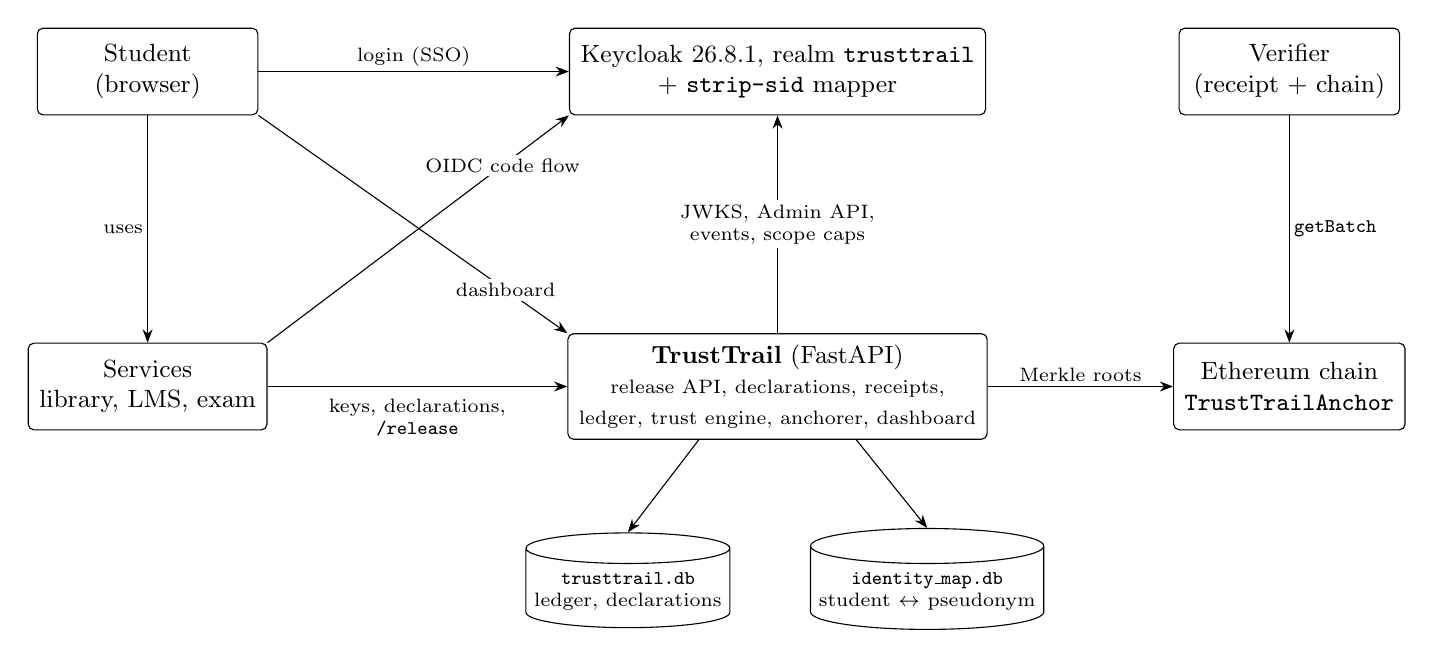
\begin{tikzpicture}[
  font=\small,
  comp/.style={draw, rounded corners=2pt, align=center, minimum height=11mm, inner sep=4pt},
  store/.style={draw, cylinder, shape border rotate=90, aspect=0.15, align=center, minimum height=9mm, inner sep=3pt, font=\scriptsize},
  lab/.style={font=\scriptsize, align=center, fill=white, inner sep=1.5pt},
  arr/.style={-{Stealth}}]
\node[comp, minimum width=28mm] (student) at (-1.5,0) {Student\\(browser)};
\node[comp, minimum width=40mm] (kc) at (6.5,0) {Keycloak 26.8.1, realm \code{trusttrail}\\+ \code{strip-sid} mapper};
\node[comp, minimum width=28mm] (ver) at (13,0) {Verifier\\(receipt + chain)};
\node[comp, minimum width=28mm] (svc) at (-1.5,-4) {Services\\library, LMS, exam};
\node[comp, minimum width=52mm] (tt) at (6.5,-4) {\textbf{TrustTrail} (FastAPI)\\ \scriptsize release API, declarations, receipts,\\ \scriptsize ledger, trust engine, anchorer, dashboard};
\node[comp, minimum width=28mm] (chain) at (13,-4) {Ethereum chain\\\code{TrustTrailAnchor}};
\node[store] (db) at (4.6,-6.6) {\code{trusttrail.db}\\ledger, declarations};
\node[store] (map) at (8.4,-6.6) {\code{identity\_map.db}\\student $\leftrightarrow$ pseudonym};
\draw[arr] (student) -- node[lab, above] {login (SSO)} (kc);
\draw[arr] (student) -- node[lab, left] {uses} (svc);
\draw[arr] (svc.north east) -- node[lab, pos=0.78] {OIDC code flow} (kc.south west);
\draw[arr] (student.south east) -- node[lab, pos=0.8] {dashboard} (tt.north west);
\draw[arr] (svc) -- node[lab, below=1mm] {keys, declarations,\\\code{/release}} (tt);
\draw[arr] (tt) -- node[lab] {JWKS, Admin API,\\events, scope caps} (kc);
\draw[arr] (tt) -- node[lab, above] {Merkle roots} (chain);
\draw[arr] (ver) -- node[lab, right] {\code{getBatch}} (chain);
\draw[arr] (tt.south) ++(-1,0) -- (db.north);
\draw[arr] (tt.south) ++(1,0) -- (map.north);
\end{tikzpicture}
\caption{TrustTrail components. Services speak standard OIDC to Keycloak and obtain attribute values only from TrustTrail. TrustTrail keeps the student-to-pseudonym map in a separate database from the ledger, and publishes only Merkle roots to the chain.}
\label{fig:components}
\end{figure}

\subsubsection{Keycloak}
Keycloak~26.8.1 is the IdP. A seed script creates the realm \code{trusttrail} through the Admin REST API. The realm defines four client scopes, \code{profile-anonymous}, \code{profile-pseudonym}, \code{profile-partial} and \code{profile-total}, which carry no claim mappers: their only effect is to appear in the token's \code{scope} claim. Each service client has every default scope removed except \code{basic}, and has as optional scopes only the profiles up to its tier cap. Each service client also has two protocol mappers: Keycloak's SHA-256 pairwise subject mapper and TrustTrail's custom \code{trusttrail-strip-sid-mapper}, a 72-line Java class that removes the session identifier from ID and access tokens. Keycloak records only \code{LOGIN\_ERROR} events, which TrustTrail reads to detect over-cap login attempts.

\subsubsection{TrustTrail}
TrustTrail is a Python~3.12 application built with FastAPI. Its 20 modules (about 2{,}200 lines) implement:
\begin{itemize}
\item the \emph{release API}, which verifies the student's access token, the declaration and the tier cap, and returns attribute values;
\item \emph{declarations}, which verifies and stores services' signed purpose declarations and their public keys;
\item \emph{receipts}, which signs a receipt for each release with TrustTrail's ES256 key;
\item the \emph{ledger}, an append-only, hash-chained SQLite table;
\item the \emph{trust engine}, which computes each service's score and tier and applies the tier's cap to the service's Keycloak client;
\item the \emph{anchorer}, which periodically builds a Merkle tree over new ledger entries and sends its root to the contract;
\item the \emph{dashboard}, where a student logs in and sees, verifies and downloads the record of every release concerning them.
\end{itemize}
Two background threads run inside TrustTrail: the trust thread synchronises with Keycloak every 3\,s, and the anchoring thread runs every 300\,s by default.

\subsubsection{Services}
Three invented campus services, a Digital Library, a Learning System and an Examination Portal, demonstrate honest behaviour. They share one small FastAPI application (136 lines) configured by a service identifier. Three further scripted services, which we call Campus Deals, Alumni Tracker and Career Portal, each break one rule on purpose and are used in the evaluation.

\subsubsection{Chain}
A local Hardhat~3 node runs an in-memory Ethereum chain, and a one-shot container deploys the \code{TrustTrailAnchor} contract (Solidity~0.8.28) and writes its address and ABI to a deployment file that TrustTrail reads. The same contract can be deployed to the Sepolia test network by changing configuration.

\subsection{Data stores and trust boundaries}
Each party holds a different part of the state, which limits what any single compromised store reveals.
\begin{itemize}
\item \emph{Keycloak} holds the student records (name, e-mail, roll number, department, programme, year, affiliation), the client definitions and each client's random pairwise salt.
\item \emph{\code{trusttrail.db}} holds service public keys, declarations, the ledger, stored receipts, trust state, cached anchor metadata and processed event identifiers. The ledger contains attribute \emph{names}, pseudonyms and hashes, never attribute values and never a student's real user ID.
\item \emph{\code{identity\_map.db}} is a separate file that maps each (service, pseudonym) pair to the Keycloak user ID. It is needed to fetch attribute values and to show a student their own entries. Keeping it apart from the ledger means the ledger can be inspected, exported or audited without revealing who is who.
\item TrustTrail's receipt-signing key, an EC P-256 private key, is generated on first use into TrustTrail's data volume with file mode 0600. Each service's declaration-signing key is generated into a volume that only the services mount. No private key is stored in the source repository.
\item The \emph{chain} holds, per batch, a 32-byte root, the first and last entry numbers and a timestamp.
\end{itemize}

\subsection{End-to-end flow}
Figure~\ref{fig:sequence} shows the life of one release, from a service's setup to a student's verification. The steps are:
\begin{enumerate}
\item \emph{Key registration.} The service obtains a client-credentials token from Keycloak and registers its public JWK at TrustTrail.
\item \emph{Declaration.} The service signs a purpose declaration and submits it; TrustTrail verifies and stores it and returns its identifier.
\item \emph{Login.} The student opens the service, which redirects to Keycloak asking for \code{openid profile-<x>}. Keycloak authenticates the student, or reuses the SSO session, and grants the profile only if it is assigned to the client. The service exchanges the code for tokens that carry the pairwise \code{sub}, no \code{sid} and no personal claims.
\item \emph{Release.} The service calls \code{POST /release} with the student's access token and the declaration identifier. TrustTrail checks the token, the declaration, the deletion date and the tier cap, maps the pseudonym to the student, fetches the attribute values from Keycloak, and in one database transaction appends a ledger entry and signs a receipt. It returns the values and the receipt.
\item \emph{Anchoring.} At the next anchoring interval, TrustTrail computes the Merkle root of all entries since the last batch and calls \code{anchor(root, first, last)} on the contract.
\item \emph{Inspection.} The student logs in to the dashboard, sees the release, runs the verification checks and downloads a receipt bundle that can be verified later against the chain alone.
\end{enumerate}
If any check in step~4 fails, TrustTrail refuses the release. If the refusal breaks one of the three rules, TrustTrail writes a violation entry and the trust engine may lower the service's tier, which removes profile scopes from its Keycloak client.

\begin{figure}[t]
\centering
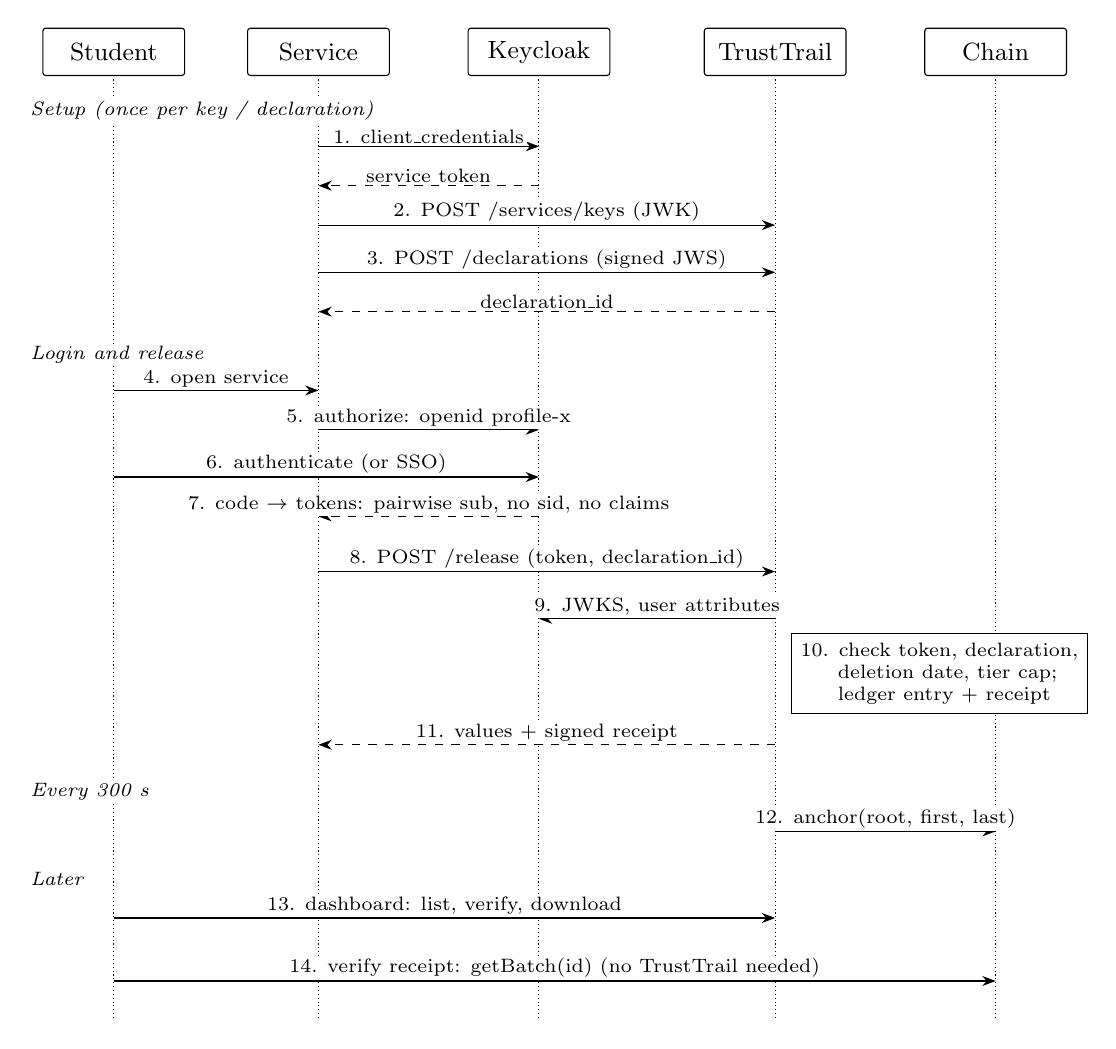
\begin{tikzpicture}[font=\scriptsize, >=Stealth]
\def\H{-12.3}
\foreach \x/\n/\t in {0/st/Student, 2.6/sv/Service, 5.4/kc/Keycloak, 8.4/tt/TrustTrail, 11.2/ch/Chain}{
  \node[draw, rounded corners=1pt, minimum width=18mm, minimum height=6mm, font=\small] (\n) at (\x,0) {\t};
  \draw[densely dotted] (\x,-0.35) -- (\x,\H);
}
\newcommand{\ttmsg}[4]{\draw[->] (#1,#3) -- node[above, align=center, font=\scriptsize, fill=white, inner sep=1pt] {#4} (#2,#3);}
\newcommand{\ttret}[4]{\draw[->, dashed] (#1,#3) -- node[above, align=center, font=\scriptsize, fill=white, inner sep=1pt] {#4} (#2,#3);}
\newcommand{\ttnote}[3]{\node[draw, fill=white, align=left, font=\scriptsize, anchor=west] at (#1,#2) {#3};}
\node[font=\scriptsize\itshape, anchor=west, fill=white, inner sep=1pt] at (-1.1,-0.75) {Setup (once per key / declaration)};
\ttmsg{2.6}{5.4}{-1.2}{1. client\_credentials}
\ttret{5.4}{2.6}{-1.7}{service token}
\ttmsg{2.6}{8.4}{-2.2}{2. POST /services/keys (JWK)}
\ttmsg{2.6}{8.4}{-2.8}{3. POST /declarations (signed JWS)}
\ttret{8.4}{2.6}{-3.3}{declaration\_id}
\node[font=\scriptsize\itshape, anchor=west, fill=white, inner sep=1pt] at (-1.1,-3.85) {Login and release};
\ttmsg{0}{2.6}{-4.3}{4. open service}
\ttmsg{2.6}{5.4}{-4.8}{5. authorize: openid profile-x}
\ttmsg{0}{5.4}{-5.4}{6. authenticate (or SSO)}
\ttret{5.4}{2.6}{-5.9}{7. code $\rightarrow$ tokens: pairwise sub, no sid, no claims}
\ttmsg{2.6}{8.4}{-6.6}{8. POST /release (token, declaration\_id)}
\ttmsg{8.4}{5.4}{-7.2}{9. JWKS, user attributes}
\ttnote{8.6}{-7.9}{10. check token, declaration,\\\ \ \ \ \ deletion date, tier cap;\\\ \ \ \ \ ledger entry + receipt}
\ttret{8.4}{2.6}{-8.8}{11. values + signed receipt}
\node[font=\scriptsize\itshape, anchor=west, fill=white, inner sep=1pt] at (-1.1,-9.4) {Every 300 s};
\ttmsg{8.4}{11.2}{-9.9}{12. anchor(root, first, last)}
\node[font=\scriptsize\itshape, anchor=west, fill=white, inner sep=1pt] at (-1.1,-10.5) {Later};
\ttmsg{0}{8.4}{-11.0}{13. dashboard: list, verify, download}
\ttmsg{0}{11.2}{-11.8}{14. verify receipt: getBatch(id) (no TrustTrail needed)}
\end{tikzpicture}
\caption{Sequence of one release, from service setup to independent verification by the student.}
\label{fig:sequence}
\end{figure}

\subsection{Deployment}
Table~\ref{tab:containers} lists the containers. Keycloak's health check gates the start of TrustTrail and the services, and TrustTrail starts only after the contract has been deployed. TrustTrail's and the services' source code is mounted into their containers, so the tests and scripts run against the code in the repository.

\begin{table}[t]
\centering
\caption{Containers in the Docker Compose deployment}
\label{tab:containers}
\small
\begin{tabularx}{\linewidth}{@{}l l X l@{}}
\toprule
Container & Image / build & Role & Port \\
\midrule
\code{keycloak} & Keycloak 26.8.1 + mapper JAR & IdP, realm \code{trusttrail} & 8080 \\
\code{chain} & Node 22, Hardhat 3 & In-memory Ethereum chain & 8545 \\
\code{chain-deploy} & same as \code{chain} & Deploys \code{TrustTrailAnchor}, writes deployment file, exits & -- \\
\code{trusttrail} & Python 3.12, FastAPI & Release API, ledger, trust, anchoring, dashboard & 8000 \\
\code{library}, \code{lms}, \code{exam} & Python 3.12, FastAPI & Honest demo services & 8001--8003 \\
\bottomrule
\end{tabularx}
\end{table}

% \section{Detailed Design}
\label{sec:design}

This section describes TrustTrail's five mechanisms in the order in which they were built: disclosure profiles and pseudonyms (\ref{sec:design-profiles}), purpose declarations and receipts (\ref{sec:design-declarations}), the ledger and dashboard (\ref{sec:design-ledger}), violations and trust (\ref{sec:design-trust}), and anchoring (\ref{sec:design-anchoring}). Section~\ref{sec:design-release} then brings them together in the release algorithm.

\subsection{Disclosure profiles, tier caps and pseudonyms}
\label{sec:design-profiles}

\subsubsection{Profiles}
TrustTrail adopts the four interaction profiles of Werner et al.~\cite{werner2015approach,werner2017survey}. Table~\ref{tab:profiles} gives the attributes that each profile releases in our deployment. The profiles are nested: each one releases everything the previous one does, plus more. The attribute vocabulary has eight names. The name \code{sub} stands for the service's pairwise pseudonym; the other seven are values from the student's Keycloak record. Profiles are defined in a configuration file, so an institute can change their contents without changing code. We keep the survey's profile names, but the \emph{anonymous} profile is not anonymous towards the service: TrustTrail releases no identifier under it, yet the service's Keycloak ID token still carries the service's pairwise \code{sub}, so the service can recognise a returning student. In the terms of Pfitzmann and Hansen~\cite{pfitzmann2010terminology} it gives relationship pseudonymity without attributes.

\begin{table}[t]
\centering
\caption{Disclosure profiles and tier caps}
\label{tab:profiles}
\small
\begin{tabularx}{\linewidth}{@{}l X l l@{}}
\toprule
Profile & Released attributes & Cap of tier & Example service (base tier) \\
\midrule
anonymous & affiliation & blocked & -- \\
pseudonym & \code{sub}, affiliation & untrusted & Digital Library \\
partial & \code{sub}, affiliation, department, program, year & semi\_trusted & Learning System \\
total & \code{sub}, affiliation, department, program, year, name, email, roll\_no & fully\_trusted & Examination Portal \\
\bottomrule
\end{tabularx}
\end{table}

\subsubsection{Tier caps at the IdP}
Each service has a \emph{base tier}, which is part of its agreement with the institute, and a \emph{current tier}, which can only be equal to or lower than the base tier (Section~\ref{sec:design-trust}). Each tier has a cap, the most revealing profile a service in that tier can obtain. TrustTrail enforces the current cap at Keycloak by assigning to the service's client exactly the optional scopes \code{profile-anonymous} up to \code{profile-}\emph{cap}. A service that asks for a profile scope that is not assigned gets an \code{invalid\_scope} error from Keycloak, and the student cannot log in to it with that request. The scopes have no claim mappers, so a granted profile only appears in the token's \code{scope} claim; it does not add any personal data to the token. To keep Keycloak from releasing personal data through its built-in scopes, the seed script removes every default scope from service clients except \code{basic}, and removes the \code{auth\_time} mapper from \code{basic}.

\subsubsection{Pairwise pseudonyms}
Every service client has Keycloak's SHA-256 pairwise subject mapper with an empty configured salt, which makes Keycloak generate a random salt per client. For a student with Keycloak user ID $u$, service sector $s$ (the host name of the service's redirect URIs) and client salt $k$, the pseudonym is
\begin{equation}
\mathit{sub}(u, s, k) = \mathrm{UUIDv3}\bigl(\mathrm{SHA\mbox{-}256}(s \,\|\, u \,\|\, k)\bigr),
\end{equation}
where $\mathrm{UUIDv3}(x)$ is Java's \code{UUID.nameUUIDFromBytes}, an MD5-based version-3 UUID of $x$. Each demo service runs under its own host name (\code{library.localhost}, \code{lms.localhost}, \code{exam.localhost}), so each is its own sector.

TrustTrail needs to map a pseudonym back to the student in order to fetch attribute values. It recomputes every student's pseudonym for a service with a port of Keycloak's algorithm, using the salt read through the Admin API, and stores the pairs in \code{identity\_map.db}. On an unknown pseudonym it rebuilds the table once. TrustTrail's service account can read the salts, so TrustTrail, and whoever controls it, can link every pseudonym to its student; this is by design, since TrustTrail must fetch the right student's attributes, and it is why the identity map is kept apart from the ledger. An integration test checks that the recomputed value equals the \code{sub} that Keycloak actually issues, for every student and every service.

\subsubsection{Removing the shared session identifier}
Pairwise identifiers alone did not give unlinkability in Keycloak~26. Keycloak adds the SSO session identifier \code{sid} to every token, and it has no built-in setting to turn this off. Every client that a student reaches within one SSO session receives the same \code{sid}. Two colluding services could therefore compare \code{sid} values and learn that pseudonym \code{f266e8cf\ldots} at the library and pseudonym \code{4336de76\ldots} at the LMS belong to the same student, which defeats the pairwise mapper.

We wrote a Keycloak protocol mapper, \code{trusttrail-strip-sid-mapper}, to remove it. It is a 72-line Java class that extends Keycloak's \code{AbstractOIDCProtocolMapper}, implements the access-token and ID-token mapper interfaces, and sets the token's session identifier to null in both. It is packaged as a JAR, built with Maven inside the Keycloak image's Docker build, and registered through Java's service loader. Two client settings remove the remaining linkable values: \code{exclude.session.state.from.auth.response=true} drops \code{session\_state} from the authorisation response, and removing the \code{auth\_time} mapper drops the exact authentication time.

Removing \code{sid} has a cost. Service tokens no longer point to a Keycloak session, so refresh tokens (which we switched off), the userinfo endpoint and logout with \code{id\_token\_hint} do not work for the service clients. TrustTrail verifies access tokens locally and is not affected. Keycloak logs a warning at start-up that the protocol mapper interface is internal and may change between versions. A browser-level check script logs in to the library and then the LMS in one SSO session, using curl as the browser, and passes only if the two \code{sub} values differ and no \code{sid}, \code{session\_state} or \code{auth\_time} reaches either service. Deleting the mapper from the two clients makes the \code{sid} check fail, which shows that the mapper is what provides this property.

\subsection{Purpose declarations and receipts}
\label{sec:design-declarations}

\subsubsection{Access tokens}
TrustTrail verifies every access token locally: the RS256 signature against Keycloak's published keys, the issuer, the expiry, and the audience. Each service client has a Keycloak audience mapper that adds \code{trusttrail} to the \code{aud} claim of its access tokens, and TrustTrail refuses any token whose audience does not include it. A valid token that Keycloak issued for some other resource server or client is therefore rejected, which follows the audience restriction recommended for OAuth resource servers~\cite{rfc8707,rfc9068}. The audience value is the same for every service, so it does not help to link students. The calling service is identified by the token's \code{azp} claim. Revocation before expiry is not checked.

\subsubsection{Service keys}
Before declaring anything, a service registers its public key. It obtains a token with the OAuth client credentials grant, using its Keycloak client secret, and calls \code{POST /services/keys} with one or more public JWKs. TrustTrail accepts only tokens that carry a \code{client\_id} claim equal to \code{azp}; Keycloak adds this claim only to client-credentials tokens, so a student's login token for the same service is rejected. This check relies on how Keycloak~26 builds its tokens. The JWT access-token profile of RFC~9068~\cite{rfc9068} makes \code{client\_id} required in all access tokens, so an IdP that follows it would need a different check, for example a dedicated audience for key registration; an integration test fails if a student's token is ever accepted. Keys must be EC or RSA, must have a \code{kid}, and must not contain private members. Our services use EC P-256 keys whose \code{kid} is the RFC~7638 thumbprint. The key registry is append-only: re-registering the same key is accepted, but reusing a \code{kid} for a different key returns \code{409 kid\_conflict}. Old declarations therefore stay verifiable forever.

\subsubsection{Declaration format and checks}
A purpose declaration is a compact JWS. Listing~\ref{lst:declaration} shows the header and payload of the LMS's declaration. The header must have \code{typ} equal to \code{purpose-declaration+jwt}, so that no other kind of JWT signed with the same key can be submitted as a declaration. The payload names the service, the audience \code{trusttrail}, the attributes, a free-text purpose of at most 500 characters, the deletion date \code{retention\_until}, a fresh nonce and the validity period. A deletion date given as a calendar date means the end of that day in UTC; a timestamp with a time zone is taken exactly.

\begin{lstlisting}[caption={Header and payload of a purpose declaration (LMS)}, label={lst:declaration}]
{ "alg": "ES256", "kid": "<RFC 7638 thumbprint of the LMS key>",
  "typ": "purpose-declaration+jwt" }
{ "client_id": "lms", "aud": "trusttrail",
  "attributes": ["sub", "affiliation", "department", "program", "year"],
  "purpose": "Enrol you in the courses of your department, program and year.",
  "retention_until": "2027-05-09",
  "nonce": "<uuid4>", "iat": 1794297600, "exp": 1796889600 }
\end{lstlisting}

A service submits the JWS to \code{POST /declarations}. No bearer token is needed, because the signature authenticates the service. TrustTrail checks, in order: that the JWS parses and has the right \code{typ}; that \code{alg} is ES256 or RS256 (never \code{none} or an HMAC algorithm); that a registered key exists for the payload's \code{client\_id} and the header's \code{kid}; the signature; the audience; that the declaration is not expired and not issued in the future (with 30\,s of allowed clock skew) and is valid for at most 90 days; that the attributes are a non-empty list of known names; that the purpose is a non-empty string; and that the deletion date parses and is not already past. A nonce may be used only once per service, which stops an old declaration from being replayed as new. TrustTrail stores the declaration together with the original JWS and its SHA-256 hash, and identifies it by the first 16 hex digits of that hash. Table~\ref{tab:refusals} lists the error codes.

The key is looked up by the \code{client\_id} in the unverified payload, and the signature check then proves that the holder of that service's key signed it. A service cannot submit a declaration in another service's name without the other service's private key.

\subsubsection{Receipts}
Every successful release produces a receipt: a JWS with \code{typ} \code{release-receipt+jwt}, signed with TrustTrail's own EC P-256 key. Its payload contains the issuer, a unique identifier, the service, the profile, the names (never the values) of the released attributes, the pseudonym (only if \code{sub} was released), the purpose, the deletion date, the declaration identifier and the SHA-256 hash of the declaration's JWS, the time of release, and the number and hash of the ledger entry. TrustTrail publishes its public key at \code{/.well-known/jwks.json}.

The two signatures give two kinds of evidence. The declaration, signed by the service, shows what the service promised, and the service cannot later deny it as long as its key was not stolen. The receipt, signed by TrustTrail, shows what TrustTrail released under that promise; its \code{declaration\_sha256} binds the release to the exact declaration. A student who downloads a receipt holds evidence that does not depend on TrustTrail's database staying unchanged.

\begin{table}[t]
\centering
\caption{Refusals returned by TrustTrail}
\label{tab:refusals}
\small
\begin{tabularx}{\linewidth}{@{}l l X l@{}}
\toprule
Code & HTTP & Meaning & Violation \\
\midrule
\code{malformed}, \code{unsupported\_alg}, \code{unknown\_key} & 400 & declaration cannot be parsed, uses a forbidden algorithm or an unregistered key & -- \\
\code{bad\_signature}, \code{wrong\_audience} & 400 & declaration signature or audience is wrong & -- \\
\code{expired}, \code{not\_yet\_valid}, \code{lifetime\_too\_long} & 400 & declaration outside its validity window or valid for over 90 days & -- \\
\code{unknown\_attribute}, \code{retention\_in\_past} & 400 & names outside the vocabulary; deletion date already passed & -- \\
\code{replayed\_nonce}, \code{kid\_conflict} & 409 & nonce reused; \code{kid} reused for a different key & -- \\
\code{missing\_token}, \code{invalid\_token} & 401 & no bearer token, or token not valid & -- \\
\code{no\_declaration} & 403 & declaration missing or belongs to another service & -- \\
\code{declaration\_expired} & 403 & declaration validity has ended & -- \\
\code{retention\_passed} & 403 & request after the promised deletion date & rule 2 \\
\code{attribute\_not\_declared} & 403 & attribute not covered by the declaration & rule 1 \\
\code{attribute\_above\_tier\_cap} & 403 & attribute above the cap of the service's base tier & rule 3 \\
\code{attribute\_above\_profile} & 403 & attribute above the current (possibly lowered) profile & -- \\
\code{unknown\_subject} & 403 & pseudonym cannot be mapped to a student & -- \\
\bottomrule
\end{tabularx}
\end{table}

\subsection{The hash-chained ledger and the student dashboard}
\label{sec:design-ledger}

\subsubsection{Entry format}
Every release and every rule-breaking refusal becomes one ledger entry. Since Phase~4 there is a third kind, \code{trust\_reset}, written when an administrator forgives a service. Table~\ref{tab:ledger} lists the fields. Entries hold attribute names and the service's pseudonym for the student, never attribute values and never the student's Keycloak ID. Entry numbers are assigned by TrustTrail as $1, 2, 3, \ldots$, so a missing number is visible.

\begin{table}[t]
\centering
\caption{Ledger entry fields}
\label{tab:ledger}
\small
\begin{tabularx}{\linewidth}{@{}l X@{}}
\toprule
Field & Content \\
\midrule
\code{entry\_id} & 1, 2, 3, \ldots \\
\code{kind} & \code{release}, \code{violation} or \code{trust\_reset} \\
\code{rule} & \code{undeclared\_attribute}, \code{after\_retention}, \code{above\_tier\_cap}, or empty \\
\code{time} & UTC timestamp with microseconds \\
\code{service\_id} & the service's client ID \\
\code{student\_pseudonym} & the pairwise \code{sub} at that service (empty for resets and login-time violations) \\
\code{profile} & profile granted or requested \\
\code{attributes\_requested} & sorted names the service asked for \\
\code{attributes\_released} & sorted names released (empty for a violation) \\
\code{purpose}, \code{retention\_until}, \code{declaration\_id} & copied from the declaration (for a reset, \code{purpose} holds the reason) \\
\code{service\_signature} & the signature part of the service's declaration JWS \\
\code{prev\_hash} & \code{entry\_hash} of the previous entry; 64 zeros for entry 1 \\
\code{entry\_hash} & SHA-256 of the canonical JSON of all fields above \\
\bottomrule
\end{tabularx}
\end{table}

\subsubsection{Hash chain}
Let $e_i$ be the content of entry $i$ (all fields except \code{entry\_hash}, including \code{prev\_hash}) and $\mathrm{C}(\cdot)$ the canonical JSON encoding: keys sorted, no whitespace, UTF-8. Then
\begin{equation}
h_0 = 0^{256}, \qquad e_i.\mathit{prev\_hash} = h_{i-1}, \qquad h_i = \mathrm{SHA\mbox{-}256}\bigl(\mathrm{C}(e_i)\bigr).
\end{equation}
Because every value is a string, an integer or a sorted list of strings, this simple encoding is unambiguous without a full implementation of the JSON Canonicalization Scheme~\cite{rfc8785}. Verification walks the ledger from entry 1, recomputes each hash from the entry's content and stops at the first entry whose number, \code{prev\_hash} or content does not match. SQLite triggers abort any \code{UPDATE} or \code{DELETE} on the ledger table. The triggers only stop changes made through normal use of the database; they are not a security boundary, which is why the hash chain, the receipts and the anchors exist.

A release writes the ledger entry and stores the receipt in one database transaction. If either step fails, nothing is released. All database access goes through one lock, so concurrent releases cannot fork the chain; an integration test runs 10 releases concurrently and checks that the chain stays intact.

\subsubsection{What the chain can and cannot detect}
The chain on its own detects an entry whose content was changed and whose stored hash was left alone, an entry whose hash was recomputed (the next entry's \code{prev\_hash} no longer matches), and a deleted or reordered entry. It cannot detect two attacks by an insider who controls the whole file: rewriting an entry and recomputing every later hash, and deleting the newest entries. Both leave a chain that is internally consistent. Detecting them needs a hash that is held outside the database. Receipts and anchors provide it, and the evaluation in Section~\ref{sec:eval-tamper} tests all six cases.

\subsubsection{Student dashboard}
A student logs in to the dashboard through Keycloak with a separate client that does not use a pairwise mapper, so TrustTrail learns the student's real user ID. TrustTrail looks up the student's pseudonym at each service in \code{identity\_map.db} and shows every ledger entry whose (service, pseudonym) pair matches, newest first: the service, the profile, the attributes released or requested, the purpose and the deletion date. Violations appear as highlighted rows. For each entry, a \emph{Verify} button runs up to five checks: the entry matches its hash; the chain is intact up to this entry; the receipt is signed by TrustTrail; the receipt matches the entry; and, once the entry is anchored, its Merkle proof leads to the root stored on chain. A student can download a receipt bundle per entry, or all at once, containing the receipt, its decoded payload, TrustTrail's public key, the ledger entry, the service's original declaration JWS and the Merkle proof. A student can see only their own entries; requests for other entries return 404.

\subsection{Violations, trust score and tier demotion}
\label{sec:design-trust}

\subsubsection{The three rules}
TrustTrail can only judge behaviour that it observes. It therefore defines three violation rules, all of which concern requests:
\begin{enumerate}
\item \emph{Undeclared attribute}: an explicit request names an attribute that the declaration does not cover. Detected in \code{/release}; refused with \code{attribute\_not\_declared}.
\item \emph{After retention}: a release is requested under a declaration whose \code{retention\_until} has passed. A service that asks again after the date by which it promised to delete the data is acting outside its promise. Detected in \code{/release}; refused with \code{retention\_passed}.
\item \emph{Above tier cap}: the service asks for more than its base tier allows. At release time this is an explicit attribute request above the base cap, refused with \code{attribute\_above\_tier\_cap}. At login it is a request for a profile scope above the base cap, which Keycloak refuses with \code{invalid\_scope}. TrustTrail learns of the login case by reading Keycloak's \code{LOGIN\_ERROR} events, whose reason reads ``Invalid scopes: \ldots{} profile-total''. Each event is processed once and its identifier stored.
\end{enumerate}
Every rule break is written to the ledger as a \code{violation} entry, with the rule, what was requested and nothing released, and is returned to the service in the refusal together with the entry number.

Two refusals are deliberately \emph{not} violations. A request above the \emph{current} profile but within the base tier's cap is refused as \code{attribute\_above\_profile} without a violation. Likewise, a demoted service that asks Keycloak for a profile that its agreement allows, but its current tier does not, is refused by Keycloak but not counted. Without this distinction, a single violation would demote the service, its next ordinary request would count as another violation, and one mistake would snowball into automatic blocking.

\subsubsection{Score and tier}
A service's score is computed from facts that TrustTrail can read from Keycloak and from its own ledger:
\begin{equation}
\mathit{score} = \max\Bigl(0,\; 100 - 15\cdot[\text{no privacy policy}] - 10\cdot[\text{metadata incomplete}] - 25\cdot v\Bigr),
\end{equation}
where $[\cdot]$ is 1 if the condition holds. ``No privacy policy'' means the Keycloak client has no \code{policyUri}; ``metadata incomplete'' means any of \code{name}, \code{description}, \code{rootUrl} or \code{tosUri} is missing; $v$ is the number of violations in the last 90 days that came after the service's most recent trust reset. The tier is the base tier moved down one step for every full 25 points below 100:
\begin{equation}
d = \left\lfloor \frac{100 - \mathit{score}}{25} \right\rfloor, \qquad \mathit{tier} = \mathit{order}\bigl[\max(\mathrm{index}(\mathit{base}) - d,\; 0)\bigr],
\end{equation}
with $\mathit{order} = [\textit{blocked}, \textit{untrusted}, \textit{semi\_trusted}, \textit{fully\_trusted}]$. One violation therefore costs exactly one tier. A missing privacy policy alone (score 85) costs nothing, but together with incomplete metadata (score 75) it costs one tier. The configuration file states that every number is a starting value to tune, not a validated constant; we return to this in Section~\ref{sec:discussion}.

\subsubsection{Enforcement}
After every violation, and every 3\,s in a background thread, the trust engine recomputes each service's tier and makes Keycloak match it. It reads the service client's optional \code{profile-*} scopes through the Admin API, adds the missing ones and removes those above the cap. Because the background loop re-applies the cap continuously, a re-seeded or hand-edited Keycloak cannot silently undo a demotion. The cap is also applied a second time at release: a token issued before a demotion still carries the old profile in its \code{scope}, so \code{/release} lowers the profile to the current cap. An administrator can reset a service's trust, for example after the institute and the service have resolved a complaint; the reset is itself written to the ledger with its reason, and violations before it no longer count.

\subsection{Merkle anchoring on Ethereum}
\label{sec:design-anchoring}

\subsubsection{Batches and Merkle roots}
Every 300\,s by default, the anchoring thread asks the contract for the last anchored entry number and reads up to 5{,}000 newer entries from the ledger. If there are none, it sends no transaction. Otherwise it builds a Merkle tree over their entry hashes following RFC~6962~\cite{rfc6962}:
\begin{equation}
\mathit{leaf}_i = \mathrm{SHA\mbox{-}256}(\mathtt{0x00} \,\|\, h_i), \qquad \mathit{node} = \mathrm{SHA\mbox{-}256}(\mathtt{0x01} \,\|\, \mathit{left} \,\|\, \mathit{right}).
\end{equation}
Adjacent nodes are paired level by level; an odd node at the end of a level is promoted unchanged. Promotion avoids a weakness of duplicating the last node, with which two different batches can share a root. The thread then calls \code{anchor(root, first, last)} and waits for the transaction receipt. All entry kinds are anchored, including violations and trust resets. Figure~\ref{fig:merkle} illustrates a batch.

\begin{figure}[t]
\centering
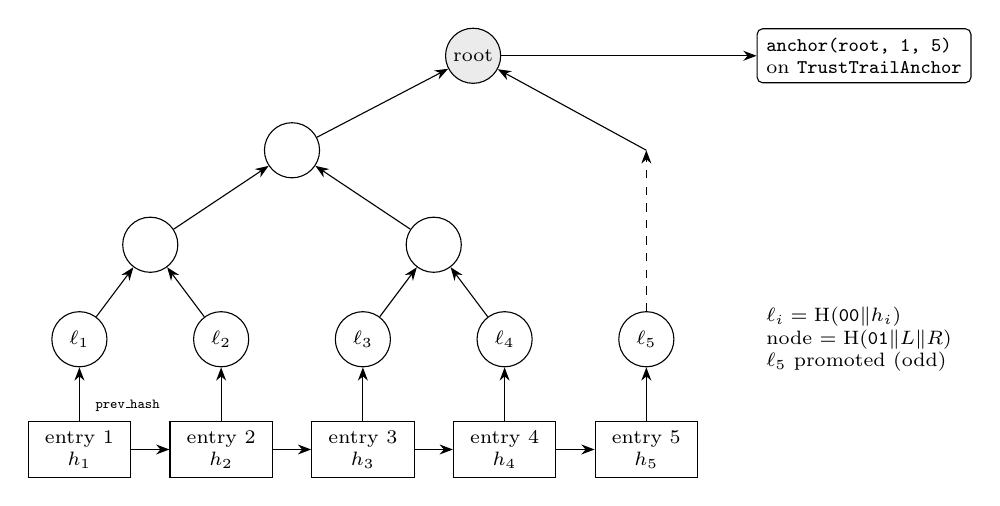
\begin{tikzpicture}[font=\scriptsize,
  e/.style={draw, minimum width=13mm, minimum height=7mm, align=center},
  n/.style={draw, circle, inner sep=1pt, minimum size=7mm},
  >=Stealth]
\foreach \i/\x in {1/0, 2/1.8, 3/3.6, 4/5.4, 5/7.2}{
  \node[e] (e\i) at (\x,0) {entry \i\\$h_{\i}$};
}
\foreach \i in {2,3,4,5}{ \pgfmathtruncatemacro{\j}{\i-1}
  \draw[->] (e\j.east) -- (e\i.west);}
\node[font=\tiny, above=0mm of e2.north west, anchor=south east] {\code{prev\_hash}};
\foreach \i/\x in {1/0, 2/1.8, 3/3.6, 4/5.4, 5/7.2}{
  \node[n] (l\i) at (\x,1.4) {$\ell_{\i}$};
  \draw[->] (e\i) -- (l\i);
}
\node[n] (n12) at (0.9,2.6) {}; \draw[->] (l1) -- (n12); \draw[->] (l2) -- (n12);
\node[n] (n34) at (4.5,2.6) {}; \draw[->] (l3) -- (n34); \draw[->] (l4) -- (n34);
\node[n] (n14) at (2.7,3.8) {}; \draw[->] (n12) -- (n14); \draw[->] (n34) -- (n14);
\draw[->, dashed] (l5) -- (7.2,3.8);
\node[n, fill=black!8] (root) at (5,5.0) {root}; \draw[->] (n14) -- (root); \draw[->] (7.2,3.8) -- (root);
\node[draw, rounded corners=2pt, align=left, anchor=west] (sc) at (8.6,5.0) {\code{anchor(root, 1, 5)}\\on \code{TrustTrailAnchor}};
\draw[->] (root) -- (sc);
\node[anchor=west, align=left] at (8.6,1.4) {$\ell_i = \mathrm{H}(\mathtt{00} \| h_i)$\\node $= \mathrm{H}(\mathtt{01} \| L \| R)$\\$\ell_5$ promoted (odd)};
\end{tikzpicture}
\caption{A batch of five hash-chained ledger entries summarised as one Merkle root and anchored on chain. The proof for entry~3 is the sibling hashes $\ell_4$, the node over $\ell_1,\ell_2$, and $\ell_5$.}
\label{fig:merkle}
\end{figure}

\subsubsection{The anchor contract}
Listing~\ref{lst:contract} shows the core of the \code{TrustTrailAnchor} contract (56 lines in total). It stores one record per batch: the root, the first and last entry numbers, and the block timestamp. Three rules make it a reliable reference. Only the owner, the account that deployed the contract and whose key TrustTrail holds, can anchor. A batch must cover at least one entry. And a batch must start exactly one entry after the previous batch ended, starting at entry~1. The last rule means the batches always cover the ledger from the first entry without gaps or overlaps, so anyone can see which entries are anchored, and a ledger that ends before the last anchored entry is visibly truncated. We deployed the contract both on a local Hardhat chain and on the Sepolia test network, at address \code{0x3415e1C6...74BC8}, where anyone can inspect its batches with a block explorer. The contract has no function that changes or deletes a batch; a contract test checks that \code{anchor} is the only function that writes state. Only hashes and numbers go on chain, never personal data.

\begin{lstlisting}[caption={Core of the anchor contract (Solidity 0.8.28)}, label={lst:contract}]
struct Batch { bytes32 root; uint64 firstEntryId; uint64 lastEntryId; uint64 anchoredAt; }
address public immutable owner;
Batch[] private batches;
event Anchored(uint256 indexed batchId, bytes32 root,
               uint64 firstEntryId, uint64 lastEntryId, uint64 anchoredAt);

function anchor(bytes32 root, uint64 firstEntryId, uint64 lastEntryId)
    external returns (uint256 batchId) {
  if (msg.sender != owner) revert NotOwner();
  if (lastEntryId < firstEntryId) revert EmptyRange();
  uint64 expected = batches.length == 0 ? 1 : batches[batches.length - 1].lastEntryId + 1;
  if (firstEntryId != expected) revert NotContiguous(expected);
  batchId = batches.length;
  uint64 timestamp = uint64(block.timestamp);
  batches.push(Batch(root, firstEntryId, lastEntryId, timestamp));
  emit Anchored(batchId, root, firstEntryId, lastEntryId, timestamp);
}
\end{lstlisting}

\subsubsection{Proofs and verification}
\code{GET /ledger/proof/\{id\}} returns, for an anchored entry, its hash, the sibling hashes on the path to the root with their side, the batch, the contract address and the chain ID. It reveals no other entry's content. For an entry that is not yet anchored it returns \code{anchored: false} and the time until the next batch. \code{GET /anchors/verify} recomputes every anchored root from the ledger and compares it with the chain.

Verification always recomputes the leaf from the entry's \emph{content}, not from the stored hash, so an edited entry whose stored hash was left unchanged also fails. A student can verify a downloaded receipt bundle without contacting TrustTrail, using a script that needs only the bundle file and a chain endpoint: it checks the receipt signature, checks that the ledger entry matches the receipt, recomputes the Merkle root from the proof, reads the batch from the contract and compares the roots and the entry range.

\subsubsection{The anchoring window}
An entry is protected by its anchor only after the next batch, which is up to one interval (300\,s by default) plus the time to confirm the transaction. During this window, the entry is protected by the hash chain and by the receipt that its student may hold. The interval is a trade-off between cost (one transaction per interval when there is traffic) and the length of the window; Section~\ref{sec:eval-anchoring} measures both.

\subsection{The release algorithm}
\label{sec:design-release}

Algorithm~\ref{alg:release} brings the mechanisms together. The order of checks matters. The token and declaration are checked before anything else, so an unauthenticated caller cannot create ledger entries. The retention check comes before the attribute checks, so a service past its deletion date is told so whatever it asks for. When the service does not name attributes, TrustTrail releases the intersection of the declared attributes and the current profile, and this default request can never be a violation.

\begin{algorithm}[t]
\caption{\code{POST /release}}
\label{alg:release}
\begin{algorithmic}[1]
\Require bearer access token $t$; declaration ID $\delta$; optional attribute list $R$
\State verify $t$ with Keycloak's JWKS (RS256, issuer, audience \code{trusttrail}, type Bearer) \Comment{else 401}
\State $s \gets t.\mathit{azp}$; $D \gets$ declaration $\delta$ \Comment{else 403 \code{no\_declaration} if missing or $D.\mathit{client} \neq s$}
\State $g \gets$ highest \code{profile-*} in $t.\mathit{scope}$ (\textit{anonymous} if none)
\State $p \gets \min(g, \mathrm{cap}(\mathrm{tier}(s)))$ \Comment{tokens issued before a demotion get today's cap}
\If{$\mathit{now} > D.\mathit{exp}$} \State \Return 403 \code{declaration\_expired} \EndIf
\If{$\mathit{now} > D.\mathit{retention\_until}$} \State record violation (rule 2); \Return 403 \code{retention\_passed} \EndIf
\If{$R = \bot$} \State $A \gets D.\mathit{attributes} \cap \mathrm{attrs}(p)$
\Else
  \If{$R \not\subseteq D.\mathit{attributes}$} \State record violation (rule 1); \Return 403 \code{attribute\_not\_declared} \EndIf
  \If{$R \not\subseteq \mathrm{attrs}(\mathrm{cap}(\mathrm{base}(s)))$} \State record violation (rule 3); \Return 403 \code{attribute\_above\_tier\_cap} \EndIf
  \If{$R \not\subseteq \mathrm{attrs}(p)$} \State \Return 403 \code{attribute\_above\_profile} \Comment{no violation} \EndIf
  \State $A \gets R$
\EndIf
\State $u \gets$ student for $(s, t.\mathit{sub})$ in identity map \Comment{else 403 \code{unknown\_subject}}
\State $V \gets$ values of $A$ for $u$ from Keycloak ($\code{sub} \mapsto t.\mathit{sub}$)
\State \textbf{in one transaction:} append ledger entry; sign receipt $\rho$; store $\rho$
\State \Return $(p, V, \rho)$
\end{algorithmic}
\end{algorithm}

% \section{Implementation}
\label{sec:implementation}

We implemented TrustTrail in six phases. Each phase added one mechanism with its own tests and demonstration script: profiles and pseudonyms; declarations and receipts; the ledger and dashboard; violations and trust; anchoring; and the evaluation harness. This section describes the result. All students, services and secrets in the implementation are invented demo data.

\subsection{Technology stack}
Table~\ref{tab:stack} lists the main technologies. Keycloak suits the design because it is a widely used open-source IdP that supports pairwise identifiers, per-client scope assignment, an Admin REST API and plug-in protocol mappers. Python and FastAPI kept the TrustTrail service small. SQLite is enough for one release service at campus scale and keeps the ledger in a single file, which also made the tamper experiments easy to run on a copy. Hardhat provides a local Ethereum chain that starts in seconds, so the full system, including anchoring, runs on one laptop.

\begin{table}[t]
\centering
\caption{Technology stack}
\label{tab:stack}
\small
\begin{tabularx}{\linewidth}{@{}l l X@{}}
\toprule
Layer & Technology & Use \\
\midrule
Identity provider & Keycloak 26.8.1 & OIDC, pairwise mapper, client scopes, Admin API, events \\
Keycloak extension & Java 21, Maven & \code{trusttrail-strip-sid-mapper} (protocol mapper SPI) \\
Release service & Python 3.12, FastAPI 0.162, Uvicorn & TrustTrail API, dashboard, background threads \\
JOSE & PyJWT 2.15 (with \code{cryptography}) & token verification, declarations, receipts \\
OIDC client & Authlib 1.9 & dashboard login, demo services \\
Storage & SQLite (Python standard library) & ledger, declarations, trust state, identity map \\
Blockchain client & web3.py 7.16 & anchoring, batch reads \\
Smart contract & Solidity 0.8.28 (optimiser, 200 runs) & \code{TrustTrailAnchor} \\
Chain and tests & Hardhat 3.20, ethers 6, Mocha, Node 22 & local chain, deployment, contract tests \\
Deployment & Docker Compose & seven containers (Table~\ref{tab:containers}) \\
\bottomrule
\end{tabularx}
\end{table}

\subsection{Code organisation and size}
TrustTrail consists of 20 Python modules. The largest are the usability-study prototype (375 lines), the anchorer (179), the declaration verifier (170), the trust engine (168) and the dashboard (152). Table~\ref{tab:loc} gives the size of each part of the code base, counted with \code{wc -l} including comments and blank lines and excluding third-party code. In total the system is about 5{,}800 lines of code, of which about 1{,}200 are tests.

\begin{table}[t]
\centering
\caption{Size of the implementation}
\label{tab:loc}
\small
\begin{tabular}{@{}lrr@{}}
\toprule
Component & Files & Lines \\
\midrule
TrustTrail application (Python) & 20 & 2{,}159 \\
Dashboard page (HTML, JavaScript) & 1 & 139 \\
Scripts: seeding, demonstrations, verifiers, bad services (Python) & 9 & 1{,}025 \\
Tests (Python) & 14 & 1{,}198 \\
Evaluation harness (Python, shell) & 7 & 610 \\
Demo service application (Python) & 2 & 150 \\
Anchor contract (Solidity) & 1 & 56 \\
Deployment script, contract tests, Hardhat configuration (TypeScript) & 3 & 135 \\
Keycloak protocol mapper (Java) & 1 & 72 \\
Browser-level check scripts (shell, Python) & 3 & 224 \\
Configuration (YAML) & 7 & 255 \\
\bottomrule
\end{tabular}
\end{table}

\subsection{Configuration}
Behaviour that an institute may want to change lives in seven YAML files rather than in code: the profiles and their attributes; the services with their URLs, base tiers and declarations; the invented students; the trust tiers, score weights and synchronisation interval; the anchoring interval, maximum batch size and transaction timeout; the declaration rules (accepted algorithms, maximum lifetime of 90 days, 30\,s clock skew, 500-character purpose limit); and the usability-study scenarios. Secrets, such as client secrets, the administrator token and the anchoring key, are read from an environment file that is excluded from version control.

A seed script builds the Keycloak realm from these files through the Admin API: the four profile scopes, the service clients with their mappers and capped optional scopes, the dashboard client, the evaluation clients and the five students. The seed script deletes and recreates the realm, which makes demonstrations and tests repeatable. Re-seeding gives every client a new random pairwise salt, which changes every pseudonym and orphans existing ledger entries, so changes to a running realm are made by small idempotent scripts instead; for example, one script added the audience mapper of Section~\ref{sec:design-declarations} to the existing service clients.

\subsection{API}
Table~\ref{tab:api} summarises TrustTrail's HTTP API; Appendix~\ref{app:api} gives the full request and response formats. Endpoints that expose only hashes, scores and counts are public, so that anyone can check the ledger against the chain. Administrative endpoints require a bearer token compared in constant time.

\begin{table}[t]
\centering
\caption{TrustTrail HTTP API (summary)}
\label{tab:api}
\small
\begin{tabularx}{\linewidth}{@{}l l X@{}}
\toprule
Endpoint & Caller & Purpose \\
\midrule
\code{POST /services/keys} & service (client-credentials token) & register public signing keys \\
\code{POST /declarations} & service (signed JWS) & submit a purpose declaration \\
\code{GET /declarations/\{id\}} & public & read a stored declaration \\
\code{POST /release} & service (student's access token) & obtain attribute values and a receipt \\
\code{GET /.well-known/jwks.json} & public & TrustTrail's receipt-signing key \\
\code{GET /ledger/verify} & public & check the hash chain (no entry contents) \\
\code{GET /ledger/proof/\{id\}} & public & Merkle proof of one entry \\
\code{GET /anchors}, \code{GET /anchors/verify} & public & list batches; compare ledger with chain \\
\code{POST /anchors/run} & administrator & anchor now \\
\code{GET /trust} & public & score, tier and cap of every service \\
\code{POST /trust/sync}, \code{POST /trust/\{s\}/reset} & administrator & re-apply caps; forgive a service (recorded) \\
\code{/dashboard/...} & student (Keycloak login) & list, verify and download own entries \\
\bottomrule
\end{tabularx}
\end{table}

\subsection{Demonstration services}
The three honest services share one FastAPI application. On first use, a service generates its EC P-256 signing key into a Docker volume, registers the public key, and signs a declaration built from the configuration; it signs a fresh declaration when the current one is missing or expires within an hour. Its home page shows the declared purpose and, after login, the claims in its Keycloak ID token, the result of \code{/release} and the decoded receipt, which makes the separation between the two visible in a demonstration.

For the violation experiments, three scripted services each break exactly one rule. \emph{Campus Deals} (semi-trusted) declares only \code{sub} and \code{affiliation} but asks for department and e-mail address as well (rule~1). \emph{Alumni Tracker} (semi-trusted, and registered without a privacy policy, so its score starts at 85) declares a deletion time two seconds in the future, receives data once, waits three seconds and asks again (rule~2). \emph{Career Portal} (untrusted) asks Keycloak for the \code{profile-total} scope (rule~3). Apart from their one misbehaviour they act normally: each asks for the lower of the profile it wants and its current public cap, so a demoted service adapts to its new tier.

\subsection{Testing}
The test suite has three layers.
\begin{itemize}
\item \emph{94 unit tests} (70 test functions) run without the rest of the system: the pairwise algorithm, profile selection and the three rules, 16 cases of declaration verification (including \code{alg: none}, tampered payloads, another service's key and timestamps without a time zone), the ledger and its attacks, the trust formula, the Merkle tree with proofs for 1 to 33 leaves, ledger-against-chain verification, and the evaluation helpers.
\item \emph{57 integration tests} (43 functions) run against the seeded Docker stack, one file per phase. Among other things they check that service tokens name TrustTrail as audience and that a valid realm token issued for another client is refused, that every student has a different identifier at every service, that TrustTrail's recomputed pseudonyms match Keycloak's, that tokens carry no personal claims, that Keycloak enforces the tier cap, that a forged token is rejected, that 10 concurrent releases keep the chain intact, that each bad service is caught with the right rule and loses one tier per violation, that honest services get no violations, and that a downloaded receipt verifies against the chain and fails after its entry is edited.
\item \emph{6 contract tests} in Hardhat check that a batch is stored and the event emitted, that batches must be contiguous from entry~1, that empty ranges and non-owners are rejected, that \code{anchor} is the only state-changing function, and that anchoring a range of 100{,}000 entries does not cost more gas than the first anchor.
\end{itemize}
Three end-to-end scripts drive the real system as a user would: a browser-level SSO check (different \code{sub}, no \code{sid}, \code{session\_state} or \code{auth\_time}), a dashboard check (list, verify, download and independently verify a receipt; another student's entry returns 404), and a scripted run of the usability-study screens. All 151 Python tests and the 6 contract tests passed on 10 November 2026, with TrustTrail anchoring on Sepolia.

\subsection{Reproducibility}
The whole system starts with two commands, \code{docker compose up -d --build} followed by the seed script, and the evaluation in Section~\ref{sec:evaluation} runs with one more (\code{sh eval/run\_all.sh}, about ten minutes). Appendix~\ref{app:repro} lists the commands. The first build compiles the Keycloak mapper with Maven inside Docker and needs network access; later builds are cached.

% \section{Evaluation}
\label{sec:evaluation}

The evaluation answers the research questions of Section~\ref{sec:intro} with five experiments: a functional check of what services receive (RQ1), the cost of the privacy layer in login latency (RQ5), the detection of tampering with the ledger (RQ3), the detection of misbehaving services and the resulting change in what they receive (RQ2, RQ4), and the cost of anchoring (RQ5). It ends with a comparison against the base survey's taxonomy.

\subsection{Setup}
All experiments ran on one Apple-silicon laptop under macOS, with every component in Docker containers as in Table~\ref{tab:containers}: Keycloak~26.8.1 in development mode, TrustTrail, the three honest services and a local Hardhat chain. All data was invented: five students and six services. To exercise many logins quickly, the scripts obtain tokens with the OAuth password grant, which we enabled on the test clients for this purpose only; a browser login adds the same redirects to both variants we compare. The latency, tamper and violation experiments are scripted in TrustTrail's evaluation harness and were run on 10 November 2026 with \code{eval/run\_all.sh}; the anchoring measurement was run the same day. Raw data is stored with the results.

\subsection{What services receive}
\label{sec:eval-functional}
The Phase~1 demonstration script computes, for each of the five students, the \code{sub} that each of the three services receives, and asks TrustTrail for a release on behalf of each service. In every row, the three identifiers differed. For example, student \emph{asha} is \code{f266e8cf-\ldots} at the library, \code{4336de76-\ldots} at the LMS and \code{158b3330-\ldots} at the examination portal. The Keycloak tokens received by all three services contained no personal claims. TrustTrail released \code{\{affiliation, sub\}} to the library, added department, programme and year for the LMS, and added name, e-mail address and roll number for the examination portal, exactly the profiles of Table~\ref{tab:profiles}. The script also reads each service client's assigned scopes from Keycloak: the library can obtain only \emph{anonymous} and \emph{pseudonym}, the LMS also \emph{partial}, and the examination portal all four. The browser-level check confirmed in a real authorisation code flow, with SSO between the library and the LMS, that the two services received different \code{sub} values and no \code{sid}, \code{session\_state} or \code{auth\_time}. These results come from scripted checks and the integration tests; they show that the configuration does what the design intends. They do not prove unlinkability against timing analysis, which is a non-goal.

\subsection{Latency overhead}
\label{sec:eval-latency}
\emph{Method.} We compare two ways of logging a student in to a service. The \emph{baseline} is a plain Keycloak client that receives all attributes in its ID token, the usual configuration that TrustTrail replaces; one token request completes the login. The \emph{TrustTrail} variant obtains the LMS's token (pairwise \code{sub}, no session identifier, no claims) and then calls \code{/release}, which verifies the token, applies the trust cap, checks the declaration, maps the pseudonym, fetches the attributes from Keycloak, appends a ledger entry and signs a receipt. After 10 warm-up runs of each, the harness ran 200 runs of each variant in a random interleaved order, cycling through the five students, and timed each with \code{time.perf\_counter}. Anchoring runs in the background and is not on the login path.

\emph{Results.} Table~\ref{tab:latency} and Fig.~\ref{fig:latency} show the results. The median TrustTrail login took 19.6\,ms against 16.0\,ms for the baseline, an overhead of 3.6\,ms or 22\%. At the 95th percentile the overhead was 5.5\,ms. The \code{/release} call itself had a median of 3.6\,ms. Two earlier runs of the same benchmark gave median overheads of 4.0\,ms and 3.4\,ms, so the result is stable to within about half a millisecond.

\begin{table}[t]
\centering
\caption{Login latency, 200 runs per variant (10 November 2026)}
\label{tab:latency}
\small
\begin{tabular}{@{}lrrrrr@{}}
\toprule
Variant & Median (ms) & p95 (ms) & Mean (ms) & Min (ms) & Max (ms) \\
\midrule
Plain OIDC login (no privacy layer) & 16.0 & 20.2 & 16.7 & 15.1 & 49.4 \\
TrustTrail login + release (total) & 19.6 & 25.6 & 20.1 & 17.9 & 31.0 \\
\quad of which: Keycloak token & 15.9 & 20.8 & 16.4 & 14.9 & 24.6 \\
\quad of which: TrustTrail \code{/release} & 3.6 & 5.1 & 3.8 & 2.8 & 6.4 \\
\midrule
Overhead (TrustTrail $-$ plain) & +3.6 & +5.5 & & & \\
\bottomrule
\end{tabular}
\end{table}

\begin{figure}[t]
\centering
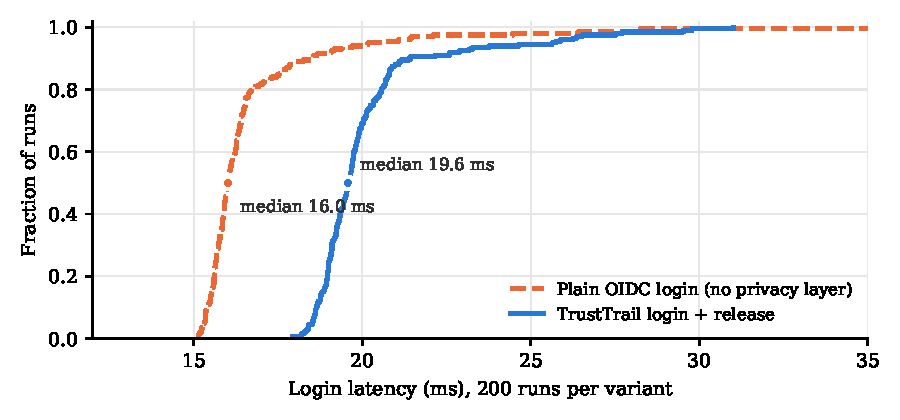
\includegraphics[width=0.85\linewidth]{figures/latency_ecdf.pdf}
\caption{Cumulative distribution of login latency. The TrustTrail curve is shifted right by the \code{/release} call, a few milliseconds. One baseline run at 49.4\,ms lies beyond the plotted range.}
\label{fig:latency}
\end{figure}

\emph{Interpretation.} The privacy layer costs a few milliseconds per login, which a user will not notice next to network and page-load times. The release call covers token verification, the declaration and cap checks, a request to Keycloak for the student record, the ledger transaction and an ECDSA signature; we did not time these steps separately. Because everything ran on one machine without network latency, the absolute numbers are lower than a deployment would see; the overhead in a deployment would also include one extra network round trip from the service to TrustTrail. We did not measure behaviour under concurrent load; all database writes go through one lock, so throughput is an open question (Section~\ref{sec:discussion}).

\subsection{Tamper detection}
\label{sec:eval-tamper}
\emph{Method.} The tamper experiment models adversary A5, an insider with write access to the database file. In each of five repetitions, the harness makes sure the ledger has at least six entries, anchors all of them, adds one more release after the anchor, and records the entry hashes contained in all stored receipts, which stand for the receipts that students have downloaded. It then picks a random target release (not the first and not the newest) and runs six attacks, each on a fresh copy of the live database with the append-only triggers dropped:
\begin{enumerate}
\item[A.] change an entry's released attributes and leave its stored hash;
\item[B.] change an entry's purpose and recompute its hash;
\item[C.] delete the entry;
\item[D.] change the entry and recompute every later hash, so the chain is consistent again;
\item[E.] cut off the tail of the ledger, from the last anchored entry onward;
\item[F.] change the release made after the last anchor and fix the hashes from there on.
\end{enumerate}
After each attack, three independent checks run: the hash chain verification, a check of every held receipt against the ledger (entry present and recomputed hash equal to the hash in the receipt), and verification of the ledger against the on-chain batches. The live ledger is never modified.

\emph{Results.} Table~\ref{tab:tamper} shows that every attack was detected by at least one check in all five repetitions, and every cell matched the outcome the design predicts. The hash chain alone missed attacks D, E and F, as Section~\ref{sec:design-ledger} explains. Receipts caught all six, because each attack changed or removed an entry for which a receipt exists. Anchoring caught all attacks on anchored entries, including D and E, which are invisible to the chain, but not attack F, which edits an entry made after the last anchor.

\begin{table}[t]
\centering
\caption{Tamper detection: repetitions in which each check detected the attack (of 5)}
\label{tab:tamper}
\small
\begin{tabular}{@{}lcccc@{}}
\toprule
Attack & Hash chain & Student receipts & Blockchain anchor & Any check \\
\midrule
A. change an entry, leave its hash & 5/5 & 5/5 & 5/5 & 5/5 \\
B. change an entry, recompute its hash & 5/5 & 5/5 & 5/5 & 5/5 \\
C. delete an entry & 5/5 & 5/5 & 5/5 & 5/5 \\
D. change an entry, recompute every later hash & 0/5 & 5/5 & 5/5 & 5/5 \\
E. cut off the tail of the ledger & 0/5 & 5/5 & 5/5 & 5/5 \\
F. change an entry made after the last anchor & 0/5 & 5/5 & 0/5 & 5/5 \\
\bottomrule
\end{tabular}
\end{table}

\emph{Interpretation.} The three mechanisms cover each other's gaps. The chain catches careless edits cheaply and locates them. Anchors catch every rewrite of anchored history, including a complete rewrite by the operator, for every student, whether or not that student kept a receipt. Receipts protect an individual student's own entries, including during the anchoring window. The one case where only receipts help, attack F, lasts at most one anchoring interval. The receipt result is optimistic in one respect: the experiment assumes students hold receipts for all affected entries, whereas in practice only students who download them do. The dashboard's own receipt check uses receipts stored by TrustTrail, which an attacker who also rewrote the receipts table would pass; only downloaded receipts are independent.

\subsection{Violation detection and trust response}
\label{sec:eval-violation}
\emph{Method.} The violation experiment models adversaries A1 and A2 with the three scripted services of Section~\ref{sec:implementation}. Each of three repetitions starts by resetting every service to its base tier (the resets are recorded in the ledger). Honest traffic comes first: each honest service receives releases for all five students twice, 30 releases per repetition. Then each bad service misbehaves five times. After each attempt the harness triggers a trust synchronisation and waits until the violation count changes, at most 15\,s, then records the score, tier and cap. An attempt counts as detected if a violation entry with the expected rule appears; a violation with another rule counts as a wrong rule; a violation recorded for an honest service is a false positive.

\emph{Results.} Table~\ref{tab:violations} shows that all 45 attempts were detected with the correct rule. Each first violation lowered the service by one tier, and the tier fell to \emph{blocked} by the second violation for the semi-trusted services and by the first for the untrusted one, after which the service could obtain only the anonymous profile. The 90 honest releases produced no violations and no tier changes. Rule~3 at login, which depends on reading Keycloak's event log, was detected as reliably as the synchronous rules.

\begin{table}[t]
\centering
\caption{Violation detection: three repetitions of five attempts per scripted service}
\label{tab:violations}
\small
\begin{tabularx}{\linewidth}{@{}l >{\raggedright\arraybackslash}X c c >{\raggedright\arraybackslash}p{4.6cm}@{}}
\toprule
Service & Misbehaviour (rule) & Detected & Wrong rule & Tier after attempts 1--5 \\
\midrule
Campus Deals & asks for attributes its declaration does not cover (1) & 15/15 & 0 & semi\_trusted $\rightarrow$ untrusted $\rightarrow$ blocked, stays blocked \\
Alumni Tracker & asks again after its deletion time (2) & 15/15 & 0 & semi\_trusted $\rightarrow$ untrusted $\rightarrow$ blocked, stays blocked \\
Career Portal & asks Keycloak for a profile above its cap (3) & 15/15 & 0 & untrusted $\rightarrow$ blocked, stays blocked \\
\midrule
Honest services & 90 releases & \multicolumn{2}{c}{0 false positives} & no tier changes \\
\bottomrule
\end{tabularx}
\end{table}

\emph{Interpretation.} The rules fire as designed and the feedback loop works: a service that breaks its promise twice is reduced to the anonymous profile within seconds, without human action, both at Keycloak and at release. The Alumni Tracker reaches \emph{blocked} after the same number of violations as Campus Deals although it starts at 85 points, because a score of 60 after one violation still means only one demotion. The 100\% detection rate is a property of scripted clients that misbehave in exactly the ways the rules describe. It does not estimate how often real services misbehave, and it says nothing about misuse after data has left TrustTrail.

\subsection{Anchoring cost and delay}
\label{sec:eval-anchoring}
\emph{Method.} The anchoring script produces a release about every 2\,s and triggers an anchor every 12\,s, for three batches, and records gas per transaction and the delay from each entry's timestamp to the confirmation of the transaction that anchors it. The contract tests measure the gas of the first anchor on a new contract and of an anchor covering a range of 100{,}000 entries.

\emph{Results.} Every anchor after the first cost 77{,}268 gas, whether it covered 6 entries, 7 entries or a range of 100{,}000 (Table~\ref{tab:gas}). The first anchor on a new contract cost 91{,}659 gas, because it initialises the batch array's storage, and deploying the contract cost 361{,}072 gas. With the 12\,s interval, the delay from entry to anchor had a median of 7.6\,s and a maximum of 12.8\,s over 19 entries; transactions were confirmed in at most 0.05\,s on the local chain.

\begin{table}[t]
\centering
\caption{Gas cost of anchoring on the local chain (10 November 2026)}
\label{tab:gas}
\small
\begin{tabular}{@{}lrr@{}}
\toprule
Operation & Entries covered & Gas \\
\midrule
Deploy \code{TrustTrailAnchor} & -- & 361{,}072 \\
First anchor on a new contract & -- & 91{,}659 \\
Later anchor (three measured batches) & 6, 6, 7 & 77{,}268 each \\
Later anchor (contract test) & 100{,}000 & 77{,}268 \\
\bottomrule
\end{tabular}
\end{table}

\emph{Interpretation.} The cost of anchoring is constant per batch, because the contract stores one 32-byte root and three numbers whatever the batch size. On a public chain the cost per batch is 77{,}268 gas multiplied by the gas price; at 1\,gwei, one anchor costs about 0.000077\,ETH, and a day of continuous traffic at the default 300\,s interval (288 anchors) about 0.022\,ETH. When nothing new is recorded, no transaction is sent. The delay scales with the interval: with the default of 300\,s, an entry waits on average about half the interval and at most one interval plus the block time, roughly 150\,s and 310\,s on a public network. These figures for a public chain are estimates from the local measurements; we did not run on Sepolia.

\subsection{Comparison with the base survey's taxonomy}
\label{sec:eval-taxonomy}
Table~\ref{tab:taxonomy} places TrustTrail in the taxonomy of Werner et al.~\cite{werner2017survey}, next to the four works in progress from the survey's Table~3. The marks for the four works are copied from the survey. The marks for TrustTrail are our own assessment, with the evidence from this paper; an assessment by authors of their own system is not independent, and we plan to have it repeated by someone who did not build TrustTrail.

\begin{table}[t]
\centering
\caption{TrustTrail and the authors' works in progress on the nine characteristics of~\cite{werner2017survey}. W1 = Weingärtner (survey ref.~[83]), W2 = Werner et al.~\cite{werner2015approach}, W3 = Bodnar et al.\ (survey ref.~[24]), W4 = Werner et al.~\cite{werner2016model}. Marks for W1--W4 are copied from the survey's Table~3 (``\checkmark'' = marked, ``p'' = partial). TrustTrail's marks are our self-assessment.}
\label{tab:taxonomy}
\small
\begin{tabularx}{\linewidth}{@{}l c c c c c >{\raggedright\arraybackslash}X@{}}
\toprule
Characteristic & W1 & W2 & W3 & W4 & TrustTrail & Evidence for TrustTrail \\
\midrule
Transparency & \checkmark & \checkmark & \checkmark & \checkmark & \checkmark & declared purpose and deletion date; dashboard lists every release and violation \\
Controllability & \checkmark & & \checkmark & \checkmark & -- & profiles set by tier, not chosen by the student; per-attribute choice only in a prototype \\
Minimization & & & & \checkmark & \checkmark & profile caps; tokens carry no claims; release = declared $\cap$ allowed \\
Accountability & & & & & \checkmark & signed declarations and receipts; hash chain; anchoring; Table~\ref{tab:tamper} \\
Data quality & \checkmark & & & & -- & IdP treated as the system of record \\
Use limitation & & & & & p & purpose and deletion date checked at every release; use after release not enforceable \\
User-friendly & & p & p & p & p & dashboard and receipts; not yet evaluated with users \\
Trust & \checkmark & & & \checkmark & p & behaviour-driven score and tier; heuristic weights \\
Obfuscation & & & & \checkmark & p & pairwise \code{sub} and no \code{sid}; anonymous profile still has a pairwise \code{sub} in the ID token \\
\bottomrule
\end{tabularx}
\end{table}

The comparison shows where TrustTrail adds to the survey's line of work: accountability and use limitation, which none of the four works address, and a trust level that follows observed behaviour. It also shows what TrustTrail gives up. The authors' works let the user choose a profile at each interaction, which counts towards controllability. TrustTrail decides the profile by the service's tier and the declaration; the student does not choose per release in the running system. Our usability-study prototype adds per-attribute choice to a consent screen, but it is not part of the evaluated system (Section~\ref{sec:future}).

\subsection{Answers to the research questions}
\begin{itemize}
\item \textbf{RQ1} (profiles and linkage): yes, with standard OIDC on the service side. Each service received only its profile's attributes, different pseudonyms, and no session identifier (Section~\ref{sec:eval-functional}); one custom Keycloak mapper was needed for the last property.
\item \textbf{RQ2} (purpose binding): yes. No release happens without a declaration signed by the service, requests outside it or after its deletion date are refused and recorded, and each release has a receipt bound to the declaration's hash.
\item \textbf{RQ3} (tamper evidence): yes, for all six attacks tried, including a full rewrite and truncation by the operator, with only hashes on chain (Table~\ref{tab:tamper}); entries newer than the last anchor rely on receipts.
\item \textbf{RQ4} (trust feedback): yes for the three observable rules; every scripted violation was detected and demoted the service, with no false positives (Table~\ref{tab:violations}).
\item \textbf{RQ5} (cost): a median of 3.6\,ms per login, and 77{,}268 gas per anchor regardless of batch size.
\end{itemize}

\subsection{Threats to validity}
\emph{Internal validity.} The latency benchmark uses the password grant, which skips the browser redirects; both variants skip them equally, but the TrustTrail variant's token request also differs slightly from the baseline's (pairwise identifier, mapper, no claim mappers). The tamper and violation experiments use attacks and clients that we wrote, and the expected outcomes were fixed in advance by the same team. \emph{External validity.} All measurements come from one laptop with local containers, invented data, five students and six services. A deployment adds network latency, more users and concurrent load. The local chain confirms transactions immediately; a public chain does not. \emph{Construct validity.} The taxonomy marks for TrustTrail are a self-assessment, and the survey's characteristics are broad enough that reasonable assessors could disagree, especially about controllability and trust.

% \section{Discussion and Limitations}
\label{sec:discussion}

\subsection{Evidence, not enforcement after release}
TrustTrail's strongest guarantees concern what happens at TrustTrail: what a service promised, what it asked for, what it received, and whether the record of these facts has been changed. It has no view of what a service does with the data afterwards. A service that stays inside its declaration but sells the data, or never deletes it, receives a perfect trust score. Rule~2 catches only a service that comes back after its deletion date. This is a limit that TrustTrail shares with every approach that releases plaintext attributes, including sticky policies without trusted hardware. What TrustTrail adds is that the service's promise is signed and recorded with each release, so that when misuse is discovered by other means, for example through a complaint, an audit or a leak, the institute and the student can show exactly what the service promised and received. In the terms of the GDPR and the DPDP Act, TrustTrail supports the controller in \emph{demonstrating} purpose limitation and accountability~\cite{gdpr2016,dpdp2023}; it does not prove storage limitation.

\subsection{Operator power and governance}
\label{sec:discussion-governance}
TrustTrail concentrates power in whoever operates it, and anchoring limits only part of that power. The operator controls what enters the ledger: a dishonest TrustTrail could release data without writing an entry, and anchoring cannot reveal a record that was never written. The receipt is the only counter-evidence, and it exists only if the student, or the service, keeps it. An anchor proves that an entry is unchanged since the anchor, not that it was true when written. The operator holds the receipt-signing key, the anchoring key and the identity map that links pseudonyms to students, and it can reset any service's trust; resets are recorded in the ledger, but nothing prevents them. In a university, the operator is usually the institute itself, which is also the Data Fiduciary responsible for the services it oversees, so TrustTrail does not create an independent auditor by itself.

Governance measures can narrow this gap, and none of them needs a change to the design. TrustTrail's administration can sit with an office that does not run the services, such as the institute's data protection or grievance officer, with separate people holding the administrator token and the anchoring key. Every administrative action that changes the record (a trust reset) is already a ledger entry, so it is anchored like any release. The anchor contract's address can be published, as we do in this paper, so that students, auditors and the services themselves can check that batches keep arriving and that the ledger they are shown matches the chain. Services also have an interest in watching: a service that keeps its own receipts can show that a release it received was recorded, and a service accused of a violation can check the entry against the chain.

\subsection{Linkability that remains}
Pairwise identifiers and the removal of \code{sid}, \code{session\_state} and \code{auth\_time} remove \emph{identifiers} that link a student across services. They do not remove timing. Two colluding services that compare the issue times of their tokens, or the network addresses of requests, could still guess which pseudonyms belong to the same student, especially in a small population. The anonymous profile is weaker than its name: TrustTrail releases no identifier under it, but the service's ID token from Keycloak still contains its pairwise \code{sub}, so the service can recognise a returning student. And Keycloak, as the IdP, sees every login. Privacy-preserving SSO protocols (Section~\ref{sec:related}) address IdP tracking and could be combined with TrustTrail.

The largest remaining channel is the released data itself. Department, programme and year together can single out a student in a small class, and the total profile releases name, e-mail address and roll number, which identify the student outright. Services that both hold such values can join their records without any identifier, so pairwise pseudonyms protect only students whose released attributes are common. The profile caps reduce this risk by giving low-trust services little to join on, but they do not remove it. Measuring it would need the size of the anonymity sets for each attribute combination in a real cohort, which we did not have.

\subsection{Is a blockchain needed?}
The anchor's job is to put the head of the ledger somewhere the operator cannot change it. A blockchain is one way to do this; Table~\ref{tab:anchor-alternatives} lists others. Each detects the same rewrites and truncations, provided the published value is kept by someone outside the operator's control. They differ in whom a verifier must trust, in cost, and in how much a verifier can check later.

\begin{table}[t]
\centering
\caption{Ways to fix the head of the ledger outside the operator's control}
\label{tab:anchor-alternatives}
\small
\begin{tabularx}{\linewidth}{@{}>{\raggedright\arraybackslash}p{3.4cm} >{\raggedright\arraybackslash}X >{\raggedright\arraybackslash}X >{\raggedright\arraybackslash}p{2.6cm}@{}}
\toprule
Option & Verifier must trust & Weakness & Cost \\
\midrule
Operator signs and publishes the head (web page, mailing list) & that someone archived the published value & the operator can replace the page; old values survive only if others kept them & none \\
Trusted timestamping authority (RFC~3161~\cite{rfc3161}) & the authority and its key & one more trusted party; tokens must be kept and the authority must stay available & low, often a paid service \\
Witnesses cosign the head (CT-style) & that enough witnesses are honest & needs independent organisations willing to run witnesses & operating cost for each witness \\
Public blockchain (TrustTrail) & the chain's consensus & fees; anchors are permanent and public; finality takes minutes & 254{,}408 gas per batch \\
\bottomrule
\end{tabularx}
\end{table}

We chose a public chain because, for a campus, it is the only option that needs no other organisation to cooperate. Anyone can check an anchor years later with nothing but a public RPC endpoint, as our receipt verifier does, and the contract itself enforces that batches are contiguous, so the operator cannot quietly skip or overlap ranges. The cost is a fee per batch and a dependence on the chain's continued operation. For an institute that already belongs to a federation with independent members, witness cosigning would be a reasonable alternative that avoids fees, and the ledger and receipts would not change.

\subsection{The ledger as personal data}
\label{sec:discussion-ledger}
The ledger contains no attribute values, but it is still personal data. Each entry records that a pseudonymous student received a service at a given time, and the identity map, held by the same operator, can link the pseudonym to the student. Under the GDPR, pseudonymised data that can be attributed to a person with additional information remains personal data (Recital~26)~\cite{gdpr2016}, and the DPDP Act's duties attach to it too~\cite{dpdp2023}. The current implementation keeps ledger entries indefinitely and offers no way to correct or erase them, which sits uneasily with the storage limitation that motivates the project and with a student's rights to correction and erasure (DPDP Act Section~12).

The append-only design does not have to conflict with erasure. Three measures fit it without weakening the tamper evidence. First, the institute can set a retention period for ledger entries, after which each expired entry is replaced by a tombstone that keeps only its number and hash, and its identity-map row is deleted. The chain links and the Merkle roots can still be checked, because they depend only on the hashes; what is lost is the ability to recompute an expired entry's hash from its content, which is acceptable once the entry has served its purpose. Second, erasure on request can be implemented by deleting the student's rows from the identity map: the ledger entries then carry pseudonyms that nobody can attribute, while their hashes, and therefore the chain and the anchors, are unchanged. Third, correction is handled by appending a correcting entry, never by editing an old one. We have not implemented these measures, and whether deleting the mapping is enough to make the remaining entries anonymous is a legal question that depends on what else the institute holds.

The anchored data needs separate thought. A Merkle root is a hash of hashes of entries, each of which contains a pseudonym and a timestamp. It reveals nothing about the entries without the ledger, and once the ledger entries and their mapping are deleted, the root is not linkable to anyone. Whether such hashes count as personal data while the ledger still exists is not settled; the European Data Protection Board has issued draft guidelines on processing personal data through blockchain technologies~\cite{edpb2025blockchain}. TrustTrail's design keeps the on-chain data to the minimum that anchoring needs, a root and an entry range, and keeps everything else off chain where it can be deleted.

\subsection{Deployment at an Indian institute}
In DPDP Act terms, the institute running TrustTrail is the Data Fiduciary, students are Data Principals, and services that the institute engages to process student data are Data Processors; a third-party service that decides its own purposes would be a Data Fiduciary in its own right. TrustTrail's records map onto several duties of the Act. The declaration and the dashboard give the student the processing purposes and the list of services that received their data, the information a Data Principal may request under Section~11. The signed deletion date gives the institute a recorded point at which the specified purpose ends, which it needs in order to apply the erasure duty of Section~8(7) to its processors. And the ledger and receipts are the evidence that a grievance under Sections~8(10) and~13 would need.

TrustTrail does not provide the remedy itself. A student who sees a violation on the dashboard needs a way to act on it, and the natural path is the institute's grievance redressal mechanism, which the Act requires anyway. A deployment would link each dashboard entry to that mechanism, so that a complaint carries the receipt and the entry number. Two further points matter in practice. The lawful basis for each service's processing, consent or one of the Act's legitimate uses, is a decision for the institute, and TrustTrail's declarations record the purpose but not the basis. And some students may be under eighteen, for whom the Act requires verifiable parental consent before processing; TrustTrail would need to know a student's age, or be configured to give such students only the lowest profiles until consent is recorded.

\subsection{Dependence on Keycloak internals}
The \code{sid} problem shows how a standard feature can undo a privacy property. Keycloak~26 adds \code{sid} to every token with no setting to turn it off, so we wrote a mapper against an SPI that Keycloak marks as internal. Its removal of \code{sid} breaks refresh tokens, the userinfo endpoint and logout with \code{id\_token\_hint} for service clients. The client setting that hides \code{session\_state} is deprecated in Keycloak~26.8; if a later version removes it, the value would return in the login redirect. Our browser-level check script fails in that case, so an upgrade that breaks the property would be noticed. Other IdPs would need equivalent configuration, and the same check, before TrustTrail could rely on them.

\subsection{The trust model}
The trust score is a heuristic. Its weights (15 points for a missing privacy policy, 10 for incomplete metadata, 25 per violation, one tier per 25 points) were chosen by hand and tested only with scripted clients. It ranks services by what TrustTrail can see, which is a narrow view of trustworthiness. Its strength is that it is simple and predictable: a service can see its own score through the public trust endpoint and knows that one violation costs one tier. Two design choices limit unfair effects. Requests within the service's agreement are never counted as violations after a demotion, so one mistake does not snowball. And violations expire after 90 days. Rule~3 at login depends on Keycloak's event log: if events are disabled or expire before TrustTrail reads them, the attempts are refused but not counted. TrustTrail's Keycloak service account holds the broad \code{manage-clients} role in order to change scope assignments; Keycloak's fine-grained admin permissions could narrow this.

\subsection{Key custody}
Non-repudiation rests on keys. A declaration binds a service only while its private key is not shared or stolen, and registering a key requires only the service's Keycloak client secret, so the client secret is the root of trust for key registration. TrustTrail's receipt key and the anchoring key are held by TrustTrail; whoever holds the anchoring key can add batches but cannot change or remove existing ones. TrustTrail checks declarations' attribute names, not the meaning of the purpose text: it cannot judge whether a stated purpose is honest or proportionate. That judgement belongs to the institute when it agrees a service's base tier.

\subsection{Scale and deployment}
The implementation targets a single campus. All database writes pass through one lock and one SQLite connection; the pseudonym map is rebuilt by reading at most 1{,}000 users per request; and we did not measure throughput under concurrent load. These are implementation limits rather than design limits: the ledger needs only an append-only table with a serialised append, which a server database provides, and the identity map can be updated incrementally. Keycloak runs in development mode, the services use the password grant for test scripts, and the local chain uses Hardhat's public test keys, so its anchors prove nothing to outsiders. We ran the anchoring on Sepolia to show that the design works on a public network. Sepolia is a test network, which its operators could in principle reset, and its gas is nearly free; a production deployment would use a main network, where fees apply (Section~\ref{sec:eval-anchoring}). Verifying many batches over a public RPC endpoint also takes time, about 18\,s for 15 batches in our run, so a verifier that checks often should cache batches it has already read.

\subsection{Lessons}
Three lessons from building TrustTrail may be useful to others. First, separating \emph{which} profile from \emph{what} it contains made the design simple: the IdP enforces the cap with a mechanism it already has, scope assignment, and the release service can be small. Second, every accountability mechanism we added closed a gap left by the previous one: the chain misses full rewrites, receipts cover only students who keep them, and anchors leave a window. None of them alone would have been enough, which matches the survey's observation that accountability is hard and under-served. Third, an automatic feedback loop needs care to be fair. Without the distinction between the base tier and the current tier, a single violation would demote a service, its next ordinary request would count as a new violation, and one mistake would end in blocking.

% \section{Future Work}
\label{sec:future}

\subsection{Usability study}
TrustTrail's transparency and user-friendliness are claims about people, which our evaluation does not test. We have designed a usability study, and its materials and analysis scripts are implemented, but it has not yet been run. It compares two consent screens: Keycloak's default consent screen, which lists scopes such as ``Email address'' and ``User profile'' with Yes and No buttons, and a TrustTrail prototype screen that shows the service's declared purpose, its trust tier, the date of its signed promise, the deletion date, the attributes that are always shared, and a checkbox for each optional attribute with nothing pre-ticked.

The design is within-subject: each participant uses both screens in two scenarios, for four tasks in total, with the order of screens and scenarios counterbalanced across four groups. In one scenario (the Learning System, semi-trusted, data kept for 180 days) the intended choice is to share department, programme and year but not e-mail address or roll number; in the other (the Examination Portal, fully trusted, 365 days) the intended choice is to share everything. Participants act as an invented student, so no real personal data is involved. For each task the study records whether the participant made the intended choice, the decision time, and whether they could correctly say which attributes the service now holds; for each screen it asks what the purpose was, how long the data will be kept, and three five-point agreement items. Comprehension will be compared between the two screens with a paired exact sign test.

Two points limit what the study can show. The per-attribute choice exists only in the prototype screen, so the study tests an interface that the running system does not yet have. And the scenario that asks for a partial share is impossible on Keycloak's screen by design, so comprehension, not choice, is the fair comparison. We plan to recruit 15 to 20 classmates after checking whether the institute requires ethics approval, and to report the study separately.

\subsection{Further directions}
\begin{itemize}
\item \emph{Student choice at release.} Bringing the prototype's per-attribute choice into the release flow would add controllability, the characteristic on which TrustTrail scores lowest against the survey's taxonomy. The declaration would then bound what a service may ask for, and the student would choose within that bound.
\item \emph{Public-chain deployment.} Deploying the anchor contract on Sepolia, and later on a public main network or a low-cost layer-2 network, would turn the anchors into evidence that outsiders can check, and allow us to measure real confirmation delays and fees.
\item \emph{Consistency proofs.} Adding Certificate Transparency's consistency proofs~\cite{rfc9162} would let a student who holds an old root check that the ledger only grew, without downloading it.
\item \emph{Selective-disclosure credentials.} Issuing attributes as verifiable credentials with selective disclosure~\cite{w3cvc2} could remove TrustTrail from the path of attribute values while keeping declarations and the ledger, and would hide the student's pseudonym map from the operator.
\item \emph{Federations with several IdPs.} Extending tiers and declarations across institutions, for example for shared library or examination services, raises the agreement questions that the survey describes for dynamic federations.
\item \emph{Independent scoring.} The taxonomy assessment in Table~\ref{tab:taxonomy} should be repeated by assessors who did not build TrustTrail.
\item \emph{Load testing and hardening.} Measuring throughput under concurrent load, moving the ledger to a server database, narrowing TrustTrail's Keycloak permissions, and running Keycloak in production mode.
\end{itemize}

% \section{Conclusion}
\label{sec:conclusion}

Single sign-on gave students one login for many services, and with it a default in which every service receives the same identifier and the same personal claims, with no stated purpose and no record. Starting from the survey of privacy strategies for identity management by Werner, Westphall and Westphall, we found that accountability and use limitation are the least covered of its nine characteristics, and that its challenge of ensuring that privacy policies are implemented remained open.

TrustTrail addresses these gaps for an OpenID Connect federation. Keycloak caps which disclosure profile each service can obtain and issues pairwise pseudonyms without a shared session identifier; TrustTrail releases attribute values only under a purpose and deletion date that the service has signed, records every release and every refused rule break in a hash-chained ledger, anchors the ledger's Merkle roots on Ethereum, and lowers the tier of services that break the rules. In our evaluation, the privacy layer added a median of 3.6\,ms to a login, all six tamper attacks were detected by at least one check, all 45 scripted violations were detected with no false positives, and each anchor after the first cost 77{,}268 gas regardless of batch size.

TrustTrail does not make a service delete data, and it does not hide logins from the identity provider. It makes the promises of services explicit, checks them at every release, and keeps a record that neither the services nor the operator can change without detection once it is anchored.

% \section*{Acknowledgment}
The authors thank their project guide, Malay Kumar, Indian Institute of Information Technology Dharwad, for guidance throughout this work.

\section*{Use of AI Tools}
The authors used Claude (Anthropic), an AI assistant, to help search for and verify related literature, extract technical facts from the project's source code, draft and edit the text of this report, and produce figures and tables. References were checked against DOI records, publisher pages or the issuing body's pages, and every number reported in the evaluation comes from the project's own measurement scripts. The authors reviewed all content and take full responsibility for it.
% TODO (authors): extend this statement if AI tools were also used to write the software.

\section*{Data and Code Availability}
All students, services, credentials and attribute values used in this work are invented; no real personal data was collected or processed. The source code, configuration, test suite, evaluation scripts and raw results (in the \code{eval/results} directory) are available from the authors on request.
% TODO (authors): replace with the repository URL if it is public.

\section*{Ethics Statement}
This work involved no human participants. The usability study described in Section~\ref{sec:future} has not been conducted; before it is, the authors will check whether approval from the institute is required and obtain informed consent from every participant.

\section*{Author Contributions}
% TODO (authors): describe each author's role, e.g. using the CRediT roles (conceptualization, software, investigation, writing).
Vijender Yadav, Ansh Hardaha and Sourabh: \textbf{[to be completed by the authors]}.

\section*{Conflict of Interest}
The authors declare no conflict of interest.

\section*{Funding}
This work received no external funding.


\bibliographystyle{IEEEtran}
\bibliography{references}

% \appendices
% \section{API Reference}
\label{app:api}

All refusals have the form \code{\{"error": "<code>", "detail": "<text>"\}}; refusals that break a rule at \code{/release} also carry \code{"violation": \{"rule", "entry\_id"\}}. Table~\ref{tab:refusals} lists the codes.

\begin{lstlisting}[caption={Requests and responses of the main endpoints}, label={lst:api}]
POST /services/keys            Authorization: Bearer <client-credentials token>
  {"keys": [{"kty":"EC","crv":"P-256","x":"...","y":"...",
             "kid":"<RFC 7638 thumbprint>","alg":"ES256","use":"sig"}]}
  -> 200 {"client_id": "lms", "kids": ["..."]}

POST /declarations             (no bearer token; the JWS signature authenticates)
  {"declaration": "<compact JWS, typ purpose-declaration+jwt>"}
  -> 201 {"declaration_id", "client_id", "nonce", "attributes", "purpose",
          "retention_until", "issued_at", "expires_at", "kid", "jws", "jws_sha256"}

POST /release                  Authorization: Bearer <student's access token>
  {"declaration_id": "226617abd0d39a21", "attributes": ["sub", "department"]}
  -> 200 {"service": "lms", "profile": "partial",
          "declaration_id": "226617abd0d39a21", "entry_id": 12,
          "released": {"sub": "97d4...", "department": "Computer Science"},
          "receipt": "<JWS, typ release-receipt+jwt>"}

GET /ledger/proof/{entry_id}
  -> {"entry_id", "anchored": true, "entry_hash",
      "proof": [{"hash", "side": "left"|"right"}, ...],
      "batch": {"batch_id", "first_entry_id", "last_entry_id", "root",
                "tx_hash", "block_number", "gas_used", "anchored_at", ...},
      "network", "chain_id", "contract"}
  -> {"entry_id", "anchored": false, "last_anchored_entry_id",
      "next_anchor_within_seconds"}              (not yet anchored)

GET /anchors/verify
  -> {"ok", "batches_checked", "anchored_up_to", "unanchored_entries",
      "failures": [{"batch_id", "reason"}]}

GET /trust
  -> {"<service>": {"score", "privacy_policy_declared", "missing_metadata",
                    "violations", "demotions", "base_tier", "tier", "cap",
                    "violations_by_rule"}, ...}
\end{lstlisting}

The receipt payload contains \code{iss}, \code{iat}, \code{jti}, \code{service}, \code{profile}, \code{attributes} (names only), \code{subject} (only if the pseudonym was released), \code{purpose}, \code{retention\_until}, \code{declaration\_id}, \code{declaration\_sha256}, \code{entry\_id}, \code{entry\_hash} and \code{released\_at}. A receipt bundle downloaded from the dashboard contains the receipt JWS and its decoded payload, TrustTrail's public key set, the ledger entry, the service's declaration JWS and the Merkle proof.

\section{Configuration Files}
\label{app:config}

\begin{lstlisting}[caption={\code{config/profiles.yaml}}, label={lst:profiles}]
order: [anonymous, pseudonym, partial, total]
profiles:
  anonymous: {sub: false, attributes: [affiliation]}
  pseudonym: {sub: true,  attributes: [affiliation]}
  partial:   {sub: true,  attributes: [affiliation, department, program, year]}
  total:     {sub: true,  attributes: [affiliation, department, program, year,
                                       name, email, roll_no]}
\end{lstlisting}

\begin{lstlisting}[caption={\code{config/trust.yaml} (comments shortened)}, label={lst:trust}]
# Every number here is a starting value to tune, not a validated constant.
tiers:
  fully_trusted: total
  semi_trusted: partial
  untrusted: pseudonym
  blocked: anonymous
tier_order: [blocked, untrusted, semi_trusted, fully_trusted]
score:
  start: 100
  no_privacy_policy: 15
  incomplete_metadata: 10
  required_metadata: [name, description, rootUrl, tosUri]
  violation_step: 25
  tier_band: 25
  violation_window_days: 90
sync_seconds: 3
\end{lstlisting}

\begin{lstlisting}[caption={\code{config/declarations.yaml} and \code{config/anchoring.yaml}}, label={lst:decl-anchor}]
audience: trusttrail
algorithms: [ES256, RS256]        # never "none" or HMAC
max_lifetime_days: 90
clock_skew_seconds: 30
max_purpose_length: 500

interval_seconds: 300             # ANCHOR_INTERVAL_SECONDS overrides
max_batch_entries: 5000
receipt_timeout_seconds: 180
\end{lstlisting}

\section{Reproducing the Results}
\label{app:repro}

\begin{lstlisting}[caption={Commands to run the system, the tests and the evaluation}, label={lst:repro}]
git clone https://github.com/desmond009/Trust-Trail.git && cd Trust-Trail
cp .env.example .env                    # local demo values only
docker compose up -d --build            # Keycloak, chain, TrustTrail, services
docker compose run --rm trusttrail python -m scripts.seed   # (re)creates the realm

docker compose exec trusttrail pytest   # 94 unit + 57 integration tests
docker compose run --rm chain-deploy npx hardhat test       # 6 contract tests
scripts/check_browser_sso.sh            # browser-level unlinkability check
scripts/check_dashboard.sh              # dashboard and receipt check

docker compose exec trusttrail sh eval/run_all.sh           # latency, tamper,
                                                            # violations (~3 min)
docker compose exec trusttrail python -m scripts.demo_phase5 \
    --batches 3 --interval 12           # anchoring gas and delay
docker compose exec trusttrail python -m scripts.verify_anchors
\end{lstlisting}


\end{document}
